\documentclass[UTF8,a4paper,12pt]{ctexart}

\usepackage{geometry}
\usepackage{graphicx}
\usepackage{float}
\usepackage{booktabs}
\usepackage{longtable}
\usepackage{array}
\usepackage{enumitem}
\usepackage{hyperref}
\usepackage{xcolor}

\newcolumntype{L}[1]{>{\raggedright\arraybackslash}p{#1}}

\geometry{
  left=2.8cm,
  right=2.8cm,
  top=2.6cm,
  bottom=2.6cm
}

\hypersetup{
  colorlinks=true,
  linkcolor=black,
  urlcolor=blue,
  citecolor=black
}

\graphicspath{{images/}}

\setlist[itemize]{leftmargin=2em}
\setlist[enumerate]{leftmargin=2em}

\newcommand{\projectname}{校园二手集市}
\newcommand{\coursename}{软件工程}
\newcommand{\teamname}{第11组}

\begin{document}

\begin{titlepage}
  \centering
  \vspace*{2cm}

  {\zihao{1}\bfseries \projectname\par}
  \vspace{1cm}
  {\zihao{2}\bfseries 最终实验报告\par}
  \vspace{2cm}

  \begin{tabular}{rl}
    课程名称： & \coursename \\
    小组名称： & \teamname \\
    项目名称： & \projectname \\
    指导教师： & 刘光迟 \\
  \end{tabular}

  \vfill

  \small
  \setlength{\tabcolsep}{4pt}
  \renewcommand{\arraystretch}{1.15}
  \begin{tabular}{L{2.5cm}L{1.8cm}L{9.9cm}}
    \toprule
    学号 & 姓名 & 角色/分工 \\
    \midrule
    09J23117 & 王朝乐 & 负责卖家端发布界面、商品管理看板、私信/留言对话框 UI 开发、状态变更交互。 \\
    09J23113 & 杨晨 & 负责买家端 UI 设计（手机浏览器适配）、商品浏览列表、关键词搜索界面、商品详情页交互实现。 \\
    09J23102 & 谌涛 & 负责数据库表结构设计（SQLite/MySQL）、订单状态机逻辑代码实现（解决超卖/并发锁定）、消息通知系统。 \\
    09J23103 & 刘一鸣 & 负责 Python Flask 框架搭建、校园统一身份认证接口对接、用户权限控制逻辑、商品增删改查 API。 \\
    09J23107 & 杨溢善 & 负责编写测试用例、单元/集成测试、性能压测、模拟异常交易场景测试、撰写用户手册。 \\
    09J23122 & 何辰玮 & 负责项目进度把控、撰写最终实验报告、组织小组讨论、协调前后端接口定义、负责总结与答辩演示。 \\
    \bottomrule
  \end{tabular}
\end{titlepage}

\pagenumbering{Roman}

\section*{摘要}
随着校园内教材、数码配件和宿舍用品等闲置物品流转需求增加，传统微信群、朋友圈和线下张贴方式存在信息分散、搜索困难、交易状态不明确和沟通记录难追踪等问题。本文围绕“校园二手集市”项目，完整记录一个面向校内学生的二手物品交易 Web 平台从立项、可行性分析、需求分析、原型设计、系统设计、程序开发到测试验收和维护规划的全过程。

系统采用前后端分离架构，前端使用 Vue 3、Vite、Vant 和 Tailwind CSS 构建移动端风格交互页面，后端使用 Spring Boot、Spring Security、JWT、Spring Data JPA 和 H2/MySQL 提供 REST API、认证鉴权、商品管理、交易状态流转、私信会话和系统通知等能力。项目实现了用户登录、资料完善、商品发布、浏览搜索、商品详情、收藏、私信、预定、取消预定、卖家确认完成和通知提醒等核心功能，形成了校园二手交易的基本闭环。

在软件工程过程方面，项目通过干系人分析确定功能和非功能需求，通过用例图、状态机图、数据流图、组件图和部署图进行建模，通过策略模式、外观模式思想和递归树形构造提升系统可扩展性，并通过自动化测试、异常场景测试、并发预定测试、前端构建和性能压测验证系统质量。最终版本能够满足课程演示和基础验收要求，并为后续扩展管理员后台、举报审核、真实校园认证和浏览器端 E2E 测试预留了方向。

\noindent\textbf{关键词：}
校园二手交易；前后端分离；Spring Boot；Vue；软件工程；测试验收

\newpage
\tableofcontents
\newpage

\pagenumbering{arabic}

\section{项目概述}

\subsection{项目背景}
在高校学习和生活场景中，学生经常需要购买或转让教材、课程资料、电子数码配件、宿舍日用品和运动用品等低价值、高频次物品。现有交易方式通常依赖班级群、二手群、朋友圈或线下熟人介绍，这些方式虽然使用门槛低，但存在信息流混乱、商品状态不透明、历史消息难检索、面交地点不统一以及沟通成本高等问题。对于买家而言，很难快速判断某件商品是否仍在售、是否距离自己较近；对于卖家而言，也需要反复回答商品是否还在、价格能否商量、在哪里面交等重复问题。

本项目正是基于这一校园内部闲置流转需求提出。与面向社会公众的大型二手平台不同，校园二手交易具有身份范围相对明确、面交距离短、交易金额较小、沟通频繁和品类集中等特点。因此，项目选择构建一个轻量化校园二手集市 Web 平台，将商品发布、搜索浏览、私信沟通、预定锁定和状态通知整合到统一系统中，提高校园闲置物品流转效率，也为课程实验提供一个较完整的软件工程实践对象。

\subsection{项目目标}
本项目目标是交付一个能够本地运行、功能闭环完整、文档和测试较为齐全的校园二手交易系统。系统面向在校学生，支持用户通过一卡通号和验证码登录，首次使用时完善昵称、宿舍地点和联系方式；卖家可以发布带图片、价格、成色、分类和面交地点的商品；买家可以浏览、搜索、收藏商品，查看详情并与卖家私信沟通；当买家确认购买意向时，可以预定商品，系统创建订单、锁定商品状态并通知卖家；交易取消或完成时，商品和订单状态同步更新。

除实现软件功能外，项目还需要体现软件工程实验的完整过程。因此，最终交付物不仅包括前后端源码，还包括可行性分析、需求规格、原型设计、用例图、状态机图、数据流图、系统架构图、组件图、部署图、安全设计、测试计划、测试用例、测试报告、用户手册、维护说明和最终报告等材料。

\subsection{系统范围}
本系统包含校园二手交易的核心信息撮合流程：用户认证、资料完善、地点选择、商品发布、图片上传、商品列表、分类筛选、关键词搜索、商品详情、收藏管理、私信会话、消息发送与撤回、商品预定、取消预定、卖家确认完成、订单列表、系统通知和未读汇总。系统默认以线下面交为交易方式，只记录商品、订单、消息和通知状态，不处理真实支付、物流配送和资金托管。

本版本不包含管理员后台、举报审核、在线支付、资金担保、物流跟踪、正式校园统一身份认证、推荐算法和大规模运营统计。这些能力被列为后续迭代方向。这样的边界设计保证项目能够在课程周期内完成并通过验收，同时保留后续扩展空间。

\subsection{小组分工}
小组按照前端、后端、数据库、测试、文档和项目管理进行分工。表 \ref{tab:team-division} 记录了各成员的学号、姓名和负责内容。

\begin{table}[H]
  \centering
  \caption{小组成员分工}
  \label{tab:team-division}
  \small
  \setlength{\tabcolsep}{4pt}
  \renewcommand{\arraystretch}{1.18}
  \begin{tabular}{L{2.5cm}L{1.9cm}L{9.8cm}}
    \toprule
    学号 & 姓名 & 负责内容 \\
    \midrule
    09J23117 & 王朝乐 & 负责卖家端发布界面、商品管理看板、私信/留言对话框 UI 开发、状态变更交互。 \\
    09J23113 & 杨晨 & 负责买家端 UI 设计（手机浏览器适配）、商品浏览列表、关键词搜索界面、商品详情页交互实现。 \\
    09J23102 & 谌涛 & 负责数据库表结构设计（SQLite/MySQL）、订单状态机逻辑代码实现（解决超卖/并发锁定）、消息通知系统。 \\
    09J23103 & 刘一鸣 & 负责 Python Flask 框架搭建、校园统一身份认证接口对接、用户权限控制逻辑、商品增删改查 API。 \\
    09J23107 & 杨溢善 & 负责编写测试用例、单元/集成测试、性能压测、模拟异常交易场景测试、撰写用户手册。 \\
    09J23122 & 何辰玮 & 负责项目进度把控、撰写最终实验报告、组织小组讨论、协调前后端接口定义、负责总结与答辩演示。 \\
    \bottomrule
  \end{tabular}
\end{table}

\section{可行性分析与项目规划}

\subsection{开发流程选择}
本项目采用以敏捷开发为主、结合阶段化评审和文档管理的混合开发流程。由于课程项目既要求最终形成可运行的软件系统，又要求在报告中完整呈现可行性分析、需求建模、界面原型、系统设计、程序开发、测试验收和维护计划，因此小组没有采用单一瀑布模型或单一敏捷模型，而是按照课程节点划分为若干开发周期，在每个周期内完成相应的软件工程活动，并通过迭代反馈不断修正需求、设计和实现。

从总体上看，项目的前期工作具有阶段化特征：小组先完成项目名称、团队分工、可行性研究、开发流程、项目进度和需求规格说明，明确系统范围、资源约束和主要风险。随后进入用户体验、系统架构、安全性和性能设计阶段，通过原型、组件图、部署图、包图等方式完善系统设计。进入编码阶段后，团队以敏捷迭代为主要方式，将系统拆分为登录认证、商品发布、商品浏览、私信通知、交易预定、状态流转、测试验收等可交付增量，持续进行前后端联调和缺陷修复。

具体开发周期如下：

\begin{enumerate}
  \item \textbf{周期一（Week5--Week7）：立项、可行性分析与需求分析。}本阶段确定项目名称和团队成员，完成可行性研究、开发流程选择、项目进度安排和需求获取/建模/规格说明。小组重点回答团队是否具备管理和技术能力、项目收益是什么、技术上是否可行、项目范围和资源预算是什么、主要风险如何降低、项目时间表如何安排、需求来自哪些利益相关者以及是否绘制场景和用例图等问题。
  \item \textbf{周期二（Week8--Week9）：用户体验设计与系统设计。}本阶段围绕前端原型、用户体验评估、前端组件划分、系统组件图、部署图、包图、安全风险和性能瓶颈展开。小组在该阶段明确移动端优先的界面方向，规划前后端分离架构，并对认证、权限、文件上传、并发预定和接口响应等安全与性能问题进行初步设计。
  \item \textbf{周期三（Week10--Week11）：设计细化与建模复核。}本阶段继续检查原型、组件图、部署图、包图、安全风险、峰值容量和性能瓶颈等内容，属于对上一周期设计结果的复核和细化。通过这一周期，小组将页面交互、系统结构和非功能需求进一步对齐，为后续编码和测试减少返工。
  \item \textbf{周期四（Week12--Week13）：程序开发、组件使用与扩展设计。}本阶段进入主要编码和实现阶段，明确开发 IDE、框架和第三方组件，分析使用现有包和组件的收益，并补充类图、对象图、顺序图和设计模式说明。同时，小组考虑后续组件变更、功能扩展和遗留代码处理方式，为项目维护和最终报告做准备。
\end{enumerate}

在每个周期内部，小组采用敏捷开发思想推进具体任务。每次迭代都会围绕一个可运行目标展开，例如先完成用户登录和资料完善，再完成商品发布与浏览，之后补齐预定、订单、私信和通知，最后集中进行测试、压测和文档整理。每个迭代都包含任务拆分、接口确认、编码、联调、反馈和修正，使系统始终保持可运行状态，并让后续需求能够根据实际演示效果进行调整。

选择这种混合流程的原因主要有以下几点：

\begin{enumerate}
  \item 课程报告要求覆盖软件工程全过程，必须保留阶段化的分析、设计、测试和维护文档。
  \item 项目开发周期较短，功能需要尽快形成可演示版本，因此需要敏捷开发的快速反馈和增量交付能力。
  \item 小组成员分别负责前端、后端、数据库、测试和文档，采用迭代方式便于并行推进并及时联调。
  \item 校园二手交易业务包含用户、商品、消息、订单和通知等多个关联模块，需求细节需要在原型验证和联调过程中逐步明确。
  \item 混合流程既能保证最终报告结构完整，也能保证系统实现过程中能够灵活调整技术方案和功能优先级。
\end{enumerate}

因此，本项目实际流程可以概括为：按照课程节点进行阶段化规划和评审，在每个阶段内部采用敏捷迭代完成可运行增量，最后通过集中测试、报告整理和答辩演示完成项目交付。

\subsubsection{流程示意图}
图 \ref{fig:hybrid-agile-process} 展示了本项目采用的混合敏捷开发流程。图中上半部分按照课程时间节点划分为四个周期，分别对应立项与需求、用户体验与系统设计、设计复核与细化、程序开发与扩展设计；图中下半部分通过迭代循环表示小组在具体实现过程中采用的敏捷开发方式。每轮迭代都从需求细化和任务拆分开始，经过编码实现、前后端联调、测试反馈和缺陷修复，最终沉淀为可运行的软件增量。

\begin{figure}[H]
  \centering
  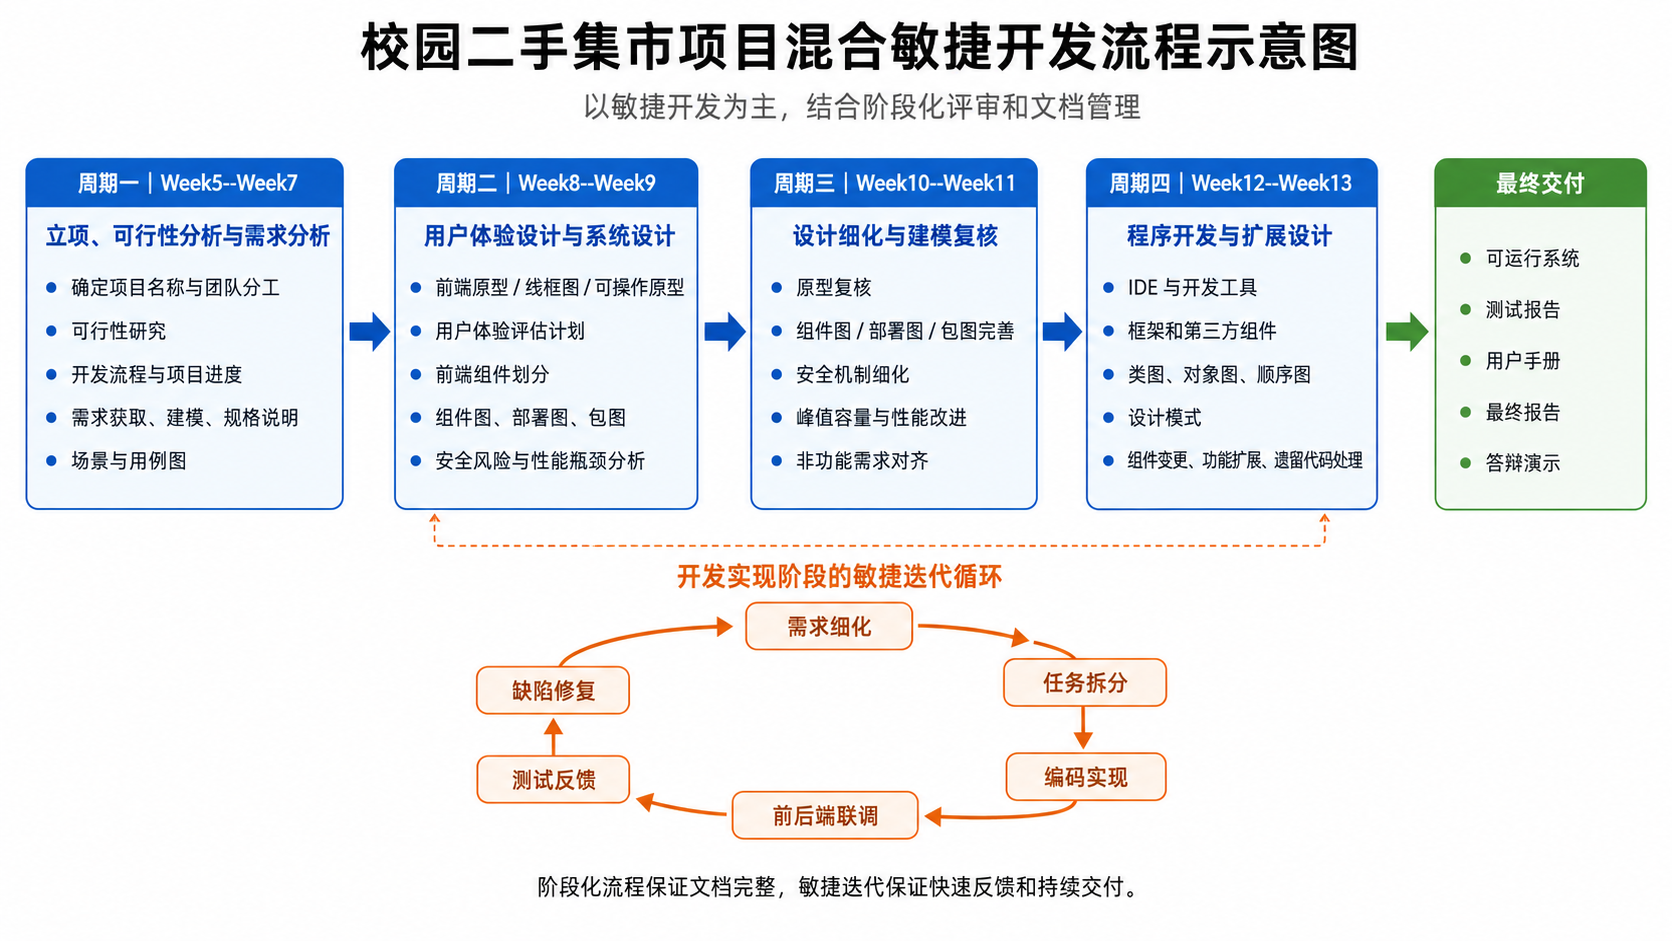
\includegraphics[width=0.95\textwidth]{liuchengtu.png}
  \caption{本项目采用的混合敏捷开发流程}
  \label{fig:hybrid-agile-process}
\end{figure}

该流程体现了本项目的两类管理需求：一方面，阶段化周期保证可行性分析、需求建模、系统设计、测试文档和最终报告等课程要求能够按节点完成；另一方面，敏捷迭代循环保证前端、后端和测试成员能够围绕可运行版本持续联调，及时根据演示效果和测试反馈调整实现细节。

\subsection{可行性分析}
本节从决策评审角度分析项目是否值得立项、是否能够完成以及是否具备持续迭代价值。评审者在本项目中可视为项目决策者，需要判断的问题不是单纯“系统能否写出来”，而是该系统面向的客户是否明确、项目边界是否可控、投入产出是否合理、技术方案是否可落地、资源估算是否匹配课程周期，以及在不实施本项目时是否存在更优替代方案。综合分析结果表明，\projectname{}面向校园内部真实交易场景，需求清晰、范围可控、收益可解释、技术路线成熟，适合作为软件工程课程实验项目实施。

\subsubsection{客户与目标用户}
本项目首先为校内学生而做，直接客户可以理解为需要完成软件工程课程实验并交付可运行系统的小组团队；最终用户则是有闲置物品交易需求的在校学生，包括买家和卖家两类核心角色。买家希望低成本获取教材、数码配件、宿舍用品等物品，卖家希望将闲置物品快速发布并在校园范围内完成可信交易。由于交易双方同属校园环境，面交地点、身份认证、沟通方式和商品类别具有较强的场景一致性，这使系统需求比面向社会公众的综合二手平台更集中，也更容易形成可验证的最小可用产品。

从决策者角度看，项目服务对象可以分为三层。第一层是学生用户，他们关注发布是否方便、浏览是否高效、交易是否可靠；第二层是课程评审者，他们关注项目是否体现需求分析、系统设计、编码实现、测试验收和维护计划等软件工程过程；第三层是学校或学院管理者，他们关注平台是否有助于校内资源循环利用、减少微信群或 QQ 群中信息混乱、诈骗风险和重复沟通成本。因此，项目并非单纯仿制通用电商平台，而是围绕校园内部低价值、高频次、轻量交易建立一个面向学生群体的小型闭环系统。

\subsubsection{项目范围与边界}
本项目范围限定为校园二手交易的核心闭环，即“用户认证--资料完善--商品发布--浏览搜索--收藏私信--预定商品--取消或完成订单--系统通知”。系统包含移动端风格前端页面、后端 REST API、数据库实体、文件上传、JWT 鉴权、测试用例和本地演示环境。项目以课程实验交付为目标，因此强调业务闭环完整、模块职责清晰和测试可验证，而不是追求商业平台的全部能力。

项目边界中明确不包含复杂支付、物流配送、资金托管、在线仲裁、管理员审核后台、推荐算法和大规模运营统计。交易方式默认采用校内线下面交，系统只负责信息撮合、预定锁定、私信沟通和状态记录，不直接处理真实资金流。举报审核、预定超时自动释放、浏览器端 E2E 测试、生产环境监控等功能被列为后续迭代方向。这样的边界设置可以避免项目膨胀，同时保证课程周期内交付一个可运行、可演示、可测试的完整版本。

\subsubsection{收益分析}
项目收益主要体现在用户收益、管理收益和课程收益三个方面。对学生用户而言，系统将原本分散在群聊、朋友圈和线下宣传中的二手信息集中到统一平台，买家可以按分类和关键词快速检索商品，卖家可以通过图片、价格、地点和描述规范发布商品，交易双方可以围绕具体商品建立私信会话，减少重复询问和信息丢失。假设一个学院或校区试点范围内有 1000 名学生，其中 30\% 每学期至少产生一次闲置交易需求，则潜在活跃用户约为 300 人；若每名活跃用户平均发布或购买 2 件商品，则单学期可支撑约 600 次商品流转。

从可量化收益看，若每次二手交易平均节省 20 元购买成本或回收 20 元闲置价值，则单学期可产生约 12000 元的学生侧经济收益。若平台将一次商品查找和沟通从微信群内反复翻找、询问的 15 分钟降低到 5 分钟，按 600 次交易估算，可节省约 6000 分钟，即约 100 小时沟通时间。对课程项目而言，收益不以软件销量为主要指标，而以功能完成度、工程过程完整性和演示验收质量衡量。若将其视为校园软件产品，初期不适合收费销售，更适合采取校内免费试点方式；在一个 5000 人规模的校区内，保守估计首学期可获得 800--1200 名注册用户、300--500 名月活用户和 1000 件左右累计发布商品。后续若接入学校统一身份认证并推广至多个校区，用户规模和交易量可进一步扩大。

\subsubsection{技术可行性}
本项目至少存在一种成熟可行的技术方案，即采用 Vue 3 + Vite + Vant 构建移动端 Web 前端，采用 Spring Boot + Spring Data JPA + Spring Security + JWT 构建后端服务，开发环境使用 H2 内存数据库，部署或扩展环境切换至 MySQL。该方案的优点是技术栈成熟、文档丰富、学习成本适中，能够覆盖用户认证、表单提交、图片上传、REST API、数据库持久化、事务处理和权限控制等需求。

从实现角度看，系统已经能够按模块拆分为认证模块、用户模块、商品模块、收藏模块、交易订单模块、私信会话模块、系统通知模块和文件上传模块。后端通过 Controller、Service、Repository、Entity 分层组织代码，前端通过路由页面、API 封装和消息状态管理组织交互。对“一物多卖”这类关键风险，技术方案中可使用数据库事务和悲观锁保证同一商品并发预定时只有一个买家成功。对开发演示和课程验收，H2 数据库可降低环境配置成本；对后续真实部署，MySQL profile 可承接正式数据存储。因此，从技术成熟度、团队掌握程度和替代实现路径来看，项目具备明确技术可行性。

\subsubsection{资源与进度可行性}
本项目资源需求与课程实验规模匹配。人员方面，建议 5--6 人小组协作：1 人负责需求分析和文档统筹，1--2 人负责前端页面与交互，1--2 人负责后端接口和数据库，1 人负责测试、联调和报告材料整理。时间方面，项目可在 Week5--Week13 的课程周期内完成：前 2--3 周完成立项、可行性分析和需求规格说明；中间 2--3 周完成原型、架构和数据库设计；后续 2--3 周完成主要编码、接口联调和功能补齐；最后 1--2 周完成测试、压测、报告整理和答辩演示。

设备和环境方面，开发只需要普通个人电脑、Java 17、Node.js、Maven、现代浏览器和 Git 版本管理工具；本地演示时后端运行在 8080 端口，前端运行在 5173 端口，无需昂贵服务器或专用硬件。若进入试点部署阶段，可使用一台 2 核 CPU、4GB 内存的云服务器运行前后端和 MySQL，图片文件存储可先使用本地上传目录，后续再迁移到对象存储。由于课程版本默认采用 H2 数据库和本地上传目录，资源约束较低，开发与演示成本可控。

\subsubsection{替代方案分析}
若不实施本项目，主要替代方案包括继续使用微信群/QQ 群发布闲置信息、使用现有社会化二手平台、使用问卷或表格收集信息、开发小程序版本，或仅完成静态原型而不实现后端系统。微信群和 QQ 群的优点是零开发成本、用户已有使用习惯，但缺点是信息流混乱、搜索困难、商品状态不明确、历史消息难以追踪，也无法体现完整的软件工程过程。社会化二手平台功能成熟，但面向全国用户，校园身份、宿舍面交、课程教材等场景适配不足，且课程实验无法体现自主分析、设计和实现能力。

使用在线表格或问卷可以低成本收集商品信息，但缺少实时浏览、收藏、私信、预定和通知能力，本质上不能形成交易闭环。开发小程序版本更贴近移动端使用习惯，但需要额外的小程序账号、审核流程和平台限制，可能增加课程周期内的不确定性。只做静态原型虽然成本最低，但无法验证接口、数据库、并发预定和测试验收等关键工程能力。综合比较后，采用 Web 前后端分离方案实现校园二手集市，是成本、周期、可演示性和工程完整性之间较均衡的选择。

\subsubsection{风险分析}
项目的主要风险集中在需求扩张、前后端联调、并发交易、测试覆盖和正式环境迁移等方面。小组通过限定项目边界、优先实现核心闭环、使用统一接口格式、编写自动化测试和保留后续迭代计划来降低风险。具体风险与应对措施见表 \ref{tab:feasibility-risk}。

\begin{table}[H]
  \centering
  \caption{项目风险分析}
  \label{tab:feasibility-risk}
  \begin{tabular}{p{2cm}p{4.2cm}p{3.2cm}p{4.5cm}}
    \toprule
    风险编号 & 风险描述 & 影响 & 应对措施 \\
    \midrule
    R1 & 功能范围持续扩大，加入支付、物流、管理员后台等非核心能力 & 延误课程周期，影响核心闭环交付 & 明确本版本只实现信息撮合、私信、预定和通知，其他能力列入后续迭代 \\
    R2 & 前后端接口字段不一致或联调时间不足 & 页面无法稳定调用后端数据 & 先约定 REST API、统一返回格式和错误码，使用接口测试提前验证后端行为 \\
    R3 & 多个买家同时预定同一商品导致一物多卖 & 破坏交易可信度，是核心业务风险 & 在交易服务中使用事务和悲观锁，并设计并发预定测试验证只有一个买家成功 \\
    R4 & 本地 H2 环境与 MySQL 正式环境存在差异 & 部署后可能出现 SQL、锁或配置问题 & 保留 MySQL profile 和 schema 文件，正式部署前在 MySQL 环境重新运行关键测试 \\
    R5 & 前端自动化测试不足，部分交互只经过手工验证 & 复杂页面可能存在遗漏缺陷 & 后续引入 Playwright E2E 测试，当前阶段通过构建验证、手工验收和后端自动化测试降低风险 \\
    \bottomrule
  \end{tabular}
\end{table}

\subsection{项目计划与进度}
项目计划以课程周为基本时间单位，以“阶段成果可评审、每轮迭代可运行”为原则制定。小组在立项阶段向课程评审者承诺：最终交付一个能够本地运行和演示的校园二手交易 Web 系统，至少覆盖登录认证、资料完善、商品发布、商品浏览与搜索、商品详情、收藏、私信、预定、取消/完成订单、系统通知等核心功能；同时提交需求分析、可行性分析、用户体验设计、系统设计、测试报告、维护说明和最终实验报告等文档成果。该承诺结果既包括软件产品本身，也包括软件工程过程材料，便于评审者从需求、设计、实现、测试和维护多个角度验收项目。

在任务拆分上，小组采用工作分解结构（WBS）将项目划分为管理与文档、前端开发、后端开发、数据库与接口、测试验收、报告整理六类工作。管理与文档任务负责确定项目范围、进度计划、需求规格和最终报告；前端任务负责登录、首页、详情、发布、消息、聊天和个人中心页面；后端任务负责认证、用户、商品、收藏、交易、消息、通知和上传接口；数据库与接口任务负责实体建模、接口字段约定和数据初始化；测试验收任务负责接口测试、异常场景测试、并发预定测试、前端构建验证和压测；报告整理任务负责将各阶段成果汇总为最终提交材料。

进度管理采用“里程碑评审 + 每周检查 + 风险缓冲”的方式进行。每个周期开始时明确本周期要回答的课程问题和要交付的材料，每周检查任务完成情况、接口阻塞点和文档缺口；若某一模块出现延期，则优先保证核心交易闭环不受影响，将管理员后台、举报审核、预定超时释放等增强功能转移到后续迭代。前后端联调采用接口优先策略：后端先提供稳定 REST API 和统一返回格式，前端基于 API 封装调用；测试人员在核心接口完成后立即补充自动化测试，避免等到项目末期才集中发现问题。

项目按照四个主要周期推进，计划与实际进度见表 \ref{tab:project-schedule}。总体来看，项目实际进展与课程节奏基本一致：前两个周期侧重立项、需求和设计，第三周期进行设计复核和接口细化，第四周期完成主要编码、测试验收和报告材料整理。由于项目范围在可行性分析阶段已经限定为校园二手交易核心闭环，因此没有出现明显范围失控；后期新增的并发预定测试、异常场景测试和性能压测也被纳入验收阶段统一处理。

\begin{table}[H]
  \centering
  \caption{项目计划与实际进度}
  \label{tab:project-schedule}
  \begin{tabular}{p{2.7cm}p{4.2cm}p{4.2cm}p{3.2cm}}
    \toprule
    阶段 & 计划任务 & 实际完成情况 & 产出物 \\
    \midrule
    Week5--Week7：立项与需求分析 & 确定项目名称、团队分工、可行性研究、开发流程、项目进度、需求获取、需求建模和规格说明 & 明确项目为校园二手集市，确定核心交易闭环和非核心功能边界，形成初步用户角色、业务场景和用例思路 & 项目概述、可行性分析、开发流程、需求说明初稿 \\
    Week8--Week9：用户体验与系统设计 & 完成前端原型、用户体验评估计划、前端组件划分、系统架构、安全性和性能设计 & 确定移动端优先的页面结构，规划 Vue 前端和 Spring Boot 后端分离架构，识别认证、上传、权限和并发预定风险 & 页面原型、组件设计、部署设计、安全与性能设计说明 \\
    Week10--Week11：设计复核与细化 & 复核原型、组件图、部署图、包图、安全风险、峰值容量和性能瓶颈 & 进一步细化商品、订单、会话、通知等模块关系，统一接口字段和状态流转规则，为编码和联调降低返工风险 & 设计图修订版、接口草案、状态流转说明 \\
    Week12--Week13：程序开发与测试验收 & 完成 IDE 与框架说明、组件使用说明、类图、对象图、顺序图、设计模式、编码实现、测试和报告整理 & 完成前后端核心功能开发，后端接口测试、异常测试、并发预定测试和前端构建验证通过，整理最终报告材料 & 可运行系统、测试报告、用户手册、维护说明、最终实验报告 \\
    \bottomrule
  \end{tabular}
\end{table}

为便于进度可视化，本项目计划使用甘特图展示各阶段任务在课程周中的分布。甘特图横轴为 Week5 到 Week13，纵轴为立项与可行性、需求分析、用户体验设计、系统设计、前端开发、后端开发、联调测试、报告整理八类任务。图中应体现前期分析与设计任务先行，前后端开发在 Week10 后并行推进，联调测试和报告整理在 Week12--Week13 集中完成，同时保留 Week13 作为缺陷修复和最终验收缓冲期。

\begin{figure}[H]
  \centering
  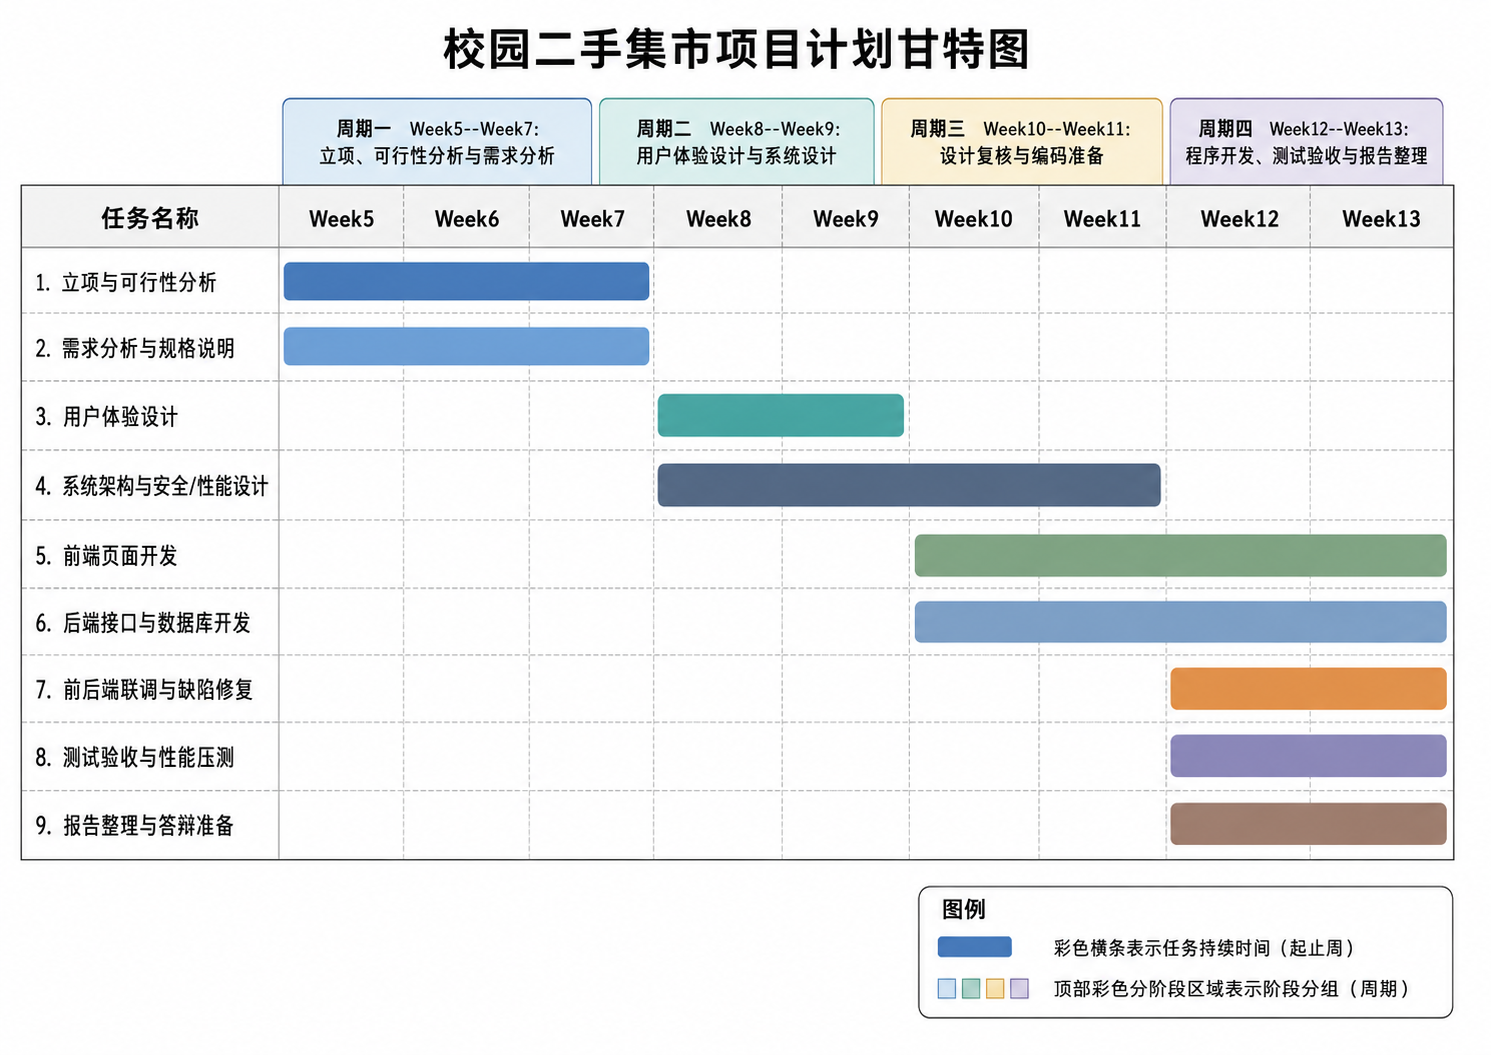
\includegraphics[width=0.95\textwidth]{Gante.png}
  \caption{项目计划甘特图}
  \label{fig:project-gantt}
\end{figure}

\section{需求分析}

\subsection{需求获取方法}
本项目的需求主要通过项目干系人分析、校园交易场景分析、小组讨论、同类产品参考和原型验证共同确定。需求获取的基本思路是：先识别谁会受到系统影响，再从每一类干系人的目标、痛点和约束出发，提炼系统必须支持的功能需求和必须满足的非功能需求。由于本项目是课程实验项目，需求必须同时满足真实用户使用价值和课程评审要求，因此小组在确定需求时遵循“核心闭环优先、可实现、可测试、可演示”的原则。

从干系人角度看，系统主要影响在校学生买家、在校学生卖家、课程评审者、小组开发成员、潜在校园管理方以及后续维护者。买家关注能否快速找到可信商品、能否和卖家沟通、能否预定并跟踪交易状态；卖家关注能否方便发布商品、管理商品状态并收到预定提醒；课程评审者关注项目是否具有完整的软件工程过程和可验证成果；开发成员关注任务边界、接口约定和进度可控；校园管理方关注平台是否降低信息混乱和交易风险；维护者关注系统是否容易部署、测试和扩展。

\begin{table}[H]
  \centering
  \caption{项目干系人与需求来源}
  \begin{tabular}{p{2.8cm}p{4.2cm}p{6.5cm}}
    \toprule
    干系人 & 主要关注点 & 导出的需求方向 \\
    \midrule
    买家学生 & 快速找到商品、判断商品是否可买、联系卖家、锁定交易机会 & 浏览搜索、商品详情、收藏、私信、预定、我的预定、系统通知 \\
    卖家学生 & 快速发布闲置、展示图片和描述、收到买家联系、避免重复交易 & 商品发布、图片上传、我的发布、订单状态流转、预定通知、完成交易 \\
    课程评审者 & 是否体现软件工程全过程，是否有可运行系统和可验证测试 & 需求文档、设计图、接口实现、测试报告、维护说明、最终报告 \\
    开发小组 & 周期有限、人员分工明确、前后端能并行开发 & 前后端分离、统一接口格式、模块化代码、里程碑计划、风险控制 \\
    校园管理方 & 交易范围可控、身份相对可信、减少公开群聊信息混乱 & 校园身份登录、线下面交地点、基础权限控制、无资金托管边界 \\
    后续维护者 & 系统能继续部署、修改和扩展 & 配置分离、H2/MySQL 两类环境、测试用例、用户手册和维护说明 \\
    \bottomrule
  \end{tabular}
\end{table}

在需求筛选过程中，小组将需求分为三类：第一类是本版本必须完成的核心需求，例如登录、发布、浏览、私信、预定和通知；第二类是提升体验但仍可在课程周期内完成的需求，例如收藏、图片预览、消息撤回、未读角标和个人中心分类列表；第三类是暂不纳入本版本的扩展需求，例如在线支付、物流配送、管理员审核后台、推荐算法和举报仲裁。这样的划分保证了需求可实现、可测试，也避免项目范围超出课程周期。

\subsection{用户角色}
根据干系人分析，系统直接使用角色主要包括未完善资料的新用户、买家用户、卖家用户和系统维护/演示人员。买家和卖家并非互斥身份，同一名学生既可以购买他人商品，也可以发布自己的闲置物品。

\begin{table}[H]
  \centering
  \caption{用户角色说明}
  \begin{tabular}{p{2.8cm}p{5cm}p{5.8cm}}
    \toprule
    用户角色 & 角色说明 & 主要目标 \\
    \midrule
    未完善资料的新用户 & 已通过一卡通号和验证码登录，但尚未填写昵称、宿舍地点和微信号的学生 & 完成个人资料，进入完整交易流程 \\
    买家用户 & 浏览并购买校园二手商品的在校学生 & 搜索商品、查看详情、收藏商品、联系卖家、预定商品、查看预定和已买到商品 \\
    卖家用户 & 发布闲置物品并与买家完成线下面交的在校学生 & 发布商品、管理自己的商品、接收私信和通知、取消或确认完成交易 \\
    系统维护/演示人员 & 负责本地运行、测试、演示和后续维护的开发成员 & 启停系统、检查数据、运行测试、维护配置和报告材料 \\
    \bottomrule
  \end{tabular}
\end{table}

\subsection{功能需求}
功能需求描述系统必须执行的功能，既包括对业务数据的增删改查，也包括用户界面中必须提供的操作入口和交互反馈。本项目功能需求按认证、用户资料、商品、交易、消息、通知和维护演示等模块编号，见表 \ref{tab:functional-requirements}。

\begin{longtable}{p{2.2cm}p{3.6cm}p{7.8cm}}
  \caption{功能需求列表}\label{tab:functional-requirements} \\
  \toprule
  编号 & 需求名称 & 需求描述 \\
  \midrule
  \endfirsthead
  \toprule
  编号 & 需求名称 & 需求描述 \\
  \midrule
  \endhead
  FR-01 & 校园身份登录 & 系统应支持用户输入 9 位一卡通号并获取验证码，验证码校验通过后生成登录状态；开发演示环境允许使用固定验证码完成登录。 \\
  FR-02 & 首次资料完善 & 系统应在新用户首次登录后引导其填写昵称、宿舍地点和微信号；未完善资料的用户不能发布商品。 \\
  FR-03 & 地点数据选择 & 系统应提供校区、苑区、楼栋等层级地点数据，供用户资料和商品面交地点选择使用。 \\
  FR-04 & 商品发布 & 卖家应能够发布商品，填写标题、分类、成色、价格、面交地点、详细描述和图片；系统应校验必填项、标题长度、价格范围和图片数量。 \\
  FR-05 & 图片上传与展示 & 系统应支持商品图片上传，限制文件类型和大小；商品列表展示封面图，详情页展示多图轮播和图片预览。 \\
  FR-06 & 商品浏览列表 & 买家应能够在首页浏览在售商品列表，列表展示标题、价格、成色、封面、卖家昵称、想要人数和地点等信息。 \\
  FR-07 & 分类筛选与关键词搜索 & 系统应支持按商品分类筛选，并支持按标题、描述或卖家昵称进行关键词搜索。 \\
  FR-08 & 商品详情查看 & 用户应能够查看商品详情，包括图片、价格、成色、描述、卖家信息、浏览量、想要人数、收藏状态和当前交易状态。 \\
  FR-09 & 商品收藏管理 & 买家应能够收藏或取消收藏商品，并在个人中心查看自己的收藏列表。 \\
  FR-10 & 我的商品与订单列表 & 用户应能够在个人中心查看我发布的商品、我预定的商品、我买到的商品和我的收藏，便于跟踪个人交易记录。 \\
  FR-11 & 私信会话创建 & 买家应能够围绕某一商品与卖家创建私信会话；系统应禁止卖家与自己发起私信。 \\
  FR-12 & 私信消息交互 & 会话参与者应能够发送文字消息、查看历史消息、引用回复消息、标记已读、删除会话，并在限定时间内撤回自己发送的消息。 \\
  FR-13 & 未读消息汇总 & 系统应统计私信和系统通知的未读数量，并在消息页和底部导航中显示角标提醒。 \\
  FR-14 & 商品预定 & 买家应能够预定在售商品；预定成功后系统创建订单、锁定商品状态为“被预定”，并自动创建或关联与卖家的会话。 \\
  FR-15 & 取消预定 & 买家或卖家应能够取消处于预定状态的订单；取消后商品恢复为“在售”，订单状态变为已取消，并通知对方。 \\
  FR-16 & 确认完成交易 & 只有卖家能够确认订单完成；完成后商品状态变为“已完成”，订单状态变为已完成，并向买家发送系统通知。 \\
  FR-17 & 系统通知 & 系统应在预定、取消预定、完成交易等事件发生时生成通知，并支持查看、单条已读和全部已读。 \\
  FR-18 & 权限与越权处理 & 系统应限制用户只能修改和删除自己发布的商品，只能查看和操作自己参与的会话及订单，并对未登录或越权操作返回明确错误。 \\
  FR-19 & 统一接口响应 & 后端 API 应使用统一响应结构返回业务数据、错误码和错误信息，便于前端展示成功、失败和空状态反馈。 \\
  FR-20 & 测试与演示支持 & 系统应支持本地 H2 数据库快速启动、开发期演示用户、接口测试和构建验证，保证课程验收时可以稳定演示。 \\
  \bottomrule
\end{longtable}

\subsection{非功能需求}
非功能需求描述系统在完成上述功能时必须满足的质量约束、组织约束和外部约束。与功能需求不同，非功能需求不直接说明“系统做什么”，而是说明系统应以怎样的质量、标准和边界来完成这些功能。本项目将非功能需求分为产品需求、组织需求、外部需求以及市场营销与公共关系需求，见表 \ref{tab:nonfunctional-requirements}。

\begin{longtable}{p{2.2cm}p{3.6cm}p{7.8cm}}
  \caption{非功能需求列表}\label{tab:nonfunctional-requirements} \\
  \toprule
  编号 & 需求类型 & 需求描述 \\
  \midrule
  \endfirsthead
  \toprule
  编号 & 需求类型 & 需求描述 \\
  \midrule
  \endhead
  NFR-01 & 性能需求 & 在课程演示和小规模试点场景下，商品列表、搜索和详情接口应在普通本地开发环境中保持秒级响应；压测目标为列表、搜索、详情接口成功率达到 100\%。 \\
  NFR-02 & 并发可靠性 & 同一商品被多个买家同时预定时，系统应保证最多只有一个买家成功预定，避免一物多卖。 \\
  NFR-03 & 可用性需求 & 前端应采用移动端优先设计，提供清晰的搜索、分类、发布、预定和消息入口；关键操作应有 Toast、空状态、加载态或禁用态反馈。 \\
  NFR-04 & 安全性需求 & 系统应使用登录令牌识别用户身份，限制未登录访问和越权操作；上传文件应限制类型和大小，避免任意文件上传风险。 \\
  NFR-05 & 数据一致性 & 预定、取消和完成交易应在事务中更新订单、商品状态和通知数据，避免状态不一致。 \\
  NFR-06 & 可靠性需求 & 后端应提供统一异常处理，业务错误不能导致服务崩溃；前端应能展示明确错误提示并保持页面可继续操作。 \\
  NFR-07 & 可维护性需求 & 后端代码应按 Controller、Service、Repository、Entity 分层组织，前端应按页面组件、API 封装和状态逻辑组织，便于后续扩展。 \\
  NFR-08 & 便携性需求 & 系统应支持本地 H2 数据库快速运行，并保留 MySQL profile 作为后续部署方案；前端应通过 Vite 构建为静态资源。 \\
  NFR-09 & 兼容性需求 & 前端应运行在现代浏览器环境中，优先适配手机尺寸页面；接口应采用 REST 风格和 JSON 数据格式，便于未来接入其他客户端。 \\
  NFR-10 & 交付要求 & 项目交付物应包括可运行源码、启动说明、测试报告、用户手册、维护说明、设计文档和最终实验报告。 \\
  NFR-11 & 培训与使用要求 & 系统应提供简明用户手册和本地运行命令，使评审者或后续维护者能够按照说明完成启动、登录、发布和交易演示。 \\
  NFR-12 & 标准与规范要求 & 代码和文档应遵循课程实验要求，接口命名、错误码、目录结构和报告章节应保持一致，避免出现难以维护的临时代码和无说明配置。 \\
  NFR-13 & 法律与隐私边界 & 系统仅收集课程演示所需的学号、昵称、宿舍地点和联系方式等基础信息，不处理真实支付和资金托管；对外展示内容应避免泄露不必要的个人隐私。 \\
  NFR-14 & 互操作性要求 & 后端应通过 HTTP API 与前端交互，上传图片通过统一路径访问；未来如接入统一身份认证或小程序端，应尽量复用现有接口。 \\
  NFR-15 & 市场营销与公共关系 & 若进行校内试点，系统宣传应强调“校园闲置流转、线下面交、降低沟通成本”，不得承诺平台提供支付担保或交易仲裁等本版本不具备的能力。 \\
  \bottomrule
\end{longtable}

\subsection{业务场景}
业务场景用于把前述功能需求放回真实使用环境中验证，重点说明典型用户在什么条件下、使用什么设备、按什么步骤完成目标。以下场景均基于校园二手交易平台的学生视角，并结合课程演示环境进行合理约束。

\subsubsection{场景一：新用户首次登录并完善资料}
\textbf{目的：}描述一名首次使用平台的在校学生如何完成身份认证和资料完善。该场景基于买家/卖家共同入口的观点，因为无论用户后续是购买还是发布商品，都必须先完成登录和基础资料设置。

\textbf{个人：}学生 A，计算机科学专业本科生，住在九龙湖校区梅园宿舍。学生 A 属于典型校园二手交易用户：拥有一卡通号，经常需要购买教材、转让课程资料或处理闲置物品。其他专业或其他校区学生也可使用该流程，只要拥有符合规则的一卡通号并能选择系统内已有的校内地点。

\textbf{设备：}学生 A 使用手机浏览器访问系统，也可以使用电脑浏览器。系统前端是 Web 页面，推荐使用现代浏览器，例如 Chrome、Edge、Safari 或手机系统自带浏览器。课程演示环境下，前端地址由开发小组提供，后端通过本地或局域网服务访问；正式部署时可通过学校或项目发布的网址进入。

\textbf{场景步骤：}
\begin{enumerate}
  \item 学生 A 打开浏览器并访问校园二手集市网址。该网址可以来自课程演示说明、班级通知或校内推广链接。
  \item 系统显示登录页，要求输入 9 位一卡通号和验证码。验证码用于模拟校园身份验证；在开发演示环境中，系统使用固定验证码以便测试。
  \item 学生 A 输入一卡通号并点击获取验证码。系统检查一卡通号格式，若格式不符合要求，则在页面中给出提示。
  \item 学生 A 输入验证码并提交登录。系统验证通过后生成登录令牌，并判断该用户是否已经完善资料。
  \item 若学生 A 是首次登录，系统自动跳转到资料完善页面。该页面要求填写昵称、宿舍地点和微信号等基础联系信息。
  \item 学生 A 通过级联选择器选择校区、苑区和楼栋。系统只提供预设的校园地点，避免用户随意填写导致面交地点不统一。
  \item 学生 A 提交资料后，系统保存用户信息并将其标记为资料已完善。此后学生 A 可以进入首页浏览商品，也可以发布自己的闲置物品。
  \item 如果学生 A 中途关闭页面或网络中断，下次重新登录后仍可继续完善资料；在资料完善前，系统应限制其进行商品发布等需要完整身份信息的操作。
\end{enumerate}

\subsubsection{场景二：卖家发布一件闲置商品}
\textbf{目的：}描述一名卖家如何将闲置物品发布到平台。该场景基于卖家学生的观点，重点验证商品数据录入、图片上传、地点选择和表单校验需求。

\textbf{个人：}学生 B，电子信息专业本科生，准备转让一台闲置蓝牙键盘。学生 B 是典型卖家：希望用较少时间发布商品，并让潜在买家看到清晰图片、价格、成色和面交地点。

\textbf{设备：}学生 B 使用手机浏览器。由于商品发布需要上传图片，设备应支持浏览器文件选择或相册选择功能。系统允许上传常见图片格式，并限制文件大小，避免非图片文件或过大文件影响系统稳定性。

\textbf{场景步骤：}
\begin{enumerate}
  \item 学生 B 登录系统并确认已完成个人资料。若资料未完善，系统先引导其完成资料填写。
  \item 学生 B 点击底部导航中的发布入口，进入“发布闲置”页面。
  \item 系统展示商品发布表单，包括图片、标题、分类、成色、价格、面交地点和详细描述等字段。
  \item 学生 B 从手机相册选择商品图片。系统上传图片并返回可访问的图片地址；若文件不是图片或超过大小限制，系统提示上传失败。
  \item 学生 B 填写商品标题，例如“九成新蓝牙键盘”，选择分类“电子数码”，选择成色“9成新”，填写价格和描述。
  \item 学生 B 选择面交地点，例如“九龙湖 / 梅园 / 2栋”。地点来自系统地点树，便于买家判断距离和面交可行性。
  \item 学生 B 点击立即发布。系统校验必填项：至少一张图片、标题不为空、分类和成色已选择、价格大于 0、地点有效。
  \item 校验通过后，系统创建商品记录，默认状态为“在售”，并跳转到商品详情页。若校验失败，系统在当前页面给出提示，保留已填写内容，方便卖家修改。
  \item 发布成功后，其他学生可以在首页列表、分类筛选或关键词搜索中看到该商品；学生 B 可以在个人中心“我发布的”列表中查看和管理它。
\end{enumerate}

\subsubsection{场景三：买家浏览、私信并预定商品}
\textbf{目的：}描述一名买家从发现商品到预定商品的完整过程。该场景基于买家学生的观点，重点验证浏览搜索、详情查看、收藏、私信、预定和通知需求。

\textbf{个人：}学生 C，软件工程专业本科生，准备购买一台二手蓝牙键盘用于宿舍学习。学生 C 是典型买家：对价格敏感，希望优先选择校内同学发布、面交地点较近且状态明确的商品。

\textbf{设备：}学生 C 使用手机浏览器访问系统。浏览和预定过程需要网络连接；若网络暂时中断，已经提交成功的操作以服务器记录为准，未提交成功的表单或请求需要重新操作。

\textbf{场景步骤：}
\begin{enumerate}
  \item 学生 C 登录系统并进入首页。系统展示当前在售商品列表，默认按发布时间展示。
  \item 学生 C 在搜索框中输入“键盘”，也可以切换到“电子数码”分类。系统返回符合关键词和分类条件的商品列表。
  \item 学生 C 点击某个商品卡片进入详情页。详情页展示商品图片、价格、成色、描述、卖家昵称、面交地点、浏览量、想要人数和当前状态。
  \item 若学生 C 暂时不决定购买，可以点击收藏。系统记录收藏关系，学生 C 后续可在个人中心“我的收藏”中再次找到该商品。
  \item 学生 C 点击“私信留言”。系统围绕该商品创建或复用买家与卖家的会话，并进入聊天页面。
  \item 学生 C 向卖家询问商品是否还在、是否可以当晚面交。系统记录消息，更新会话未读数量；卖家在消息页可以看到私信提醒。
  \item 学生 C 决定购买后返回详情页并点击“我想要”。系统弹出确认窗口，说明预定后商品会被锁定为“被预定”状态。
  \item 学生 C 确认预定。系统检查该商品是否仍处于“在售”状态，并在事务中创建订单、更新商品状态、增加想要人数和生成卖家通知。
  \item 如果另一名买家几乎同时预定同一商品，系统应通过并发控制保证只有一个买家成功；失败用户会收到“商品当前不可预定”等提示。
  \item 预定成功后，学生 C 自动进入与卖家的私信会话，继续协商面交时间和地点。卖家会收到系统通知，知道商品已被预定。
\end{enumerate}

\subsubsection{场景四：卖家确认完成或双方取消预定}
\textbf{目的：}描述商品被预定后的状态流转。该场景基于交易双方共同观点，重点验证取消预定、确认完成、订单权限和系统通知需求。

\textbf{个人：}学生 B 是卖家，学生 C 是买家。二人已经通过平台围绕同一商品建立会话，商品当前处于“被预定”状态。

\textbf{设备：}双方均使用手机浏览器。交易的实际交付发生在线下，系统只记录预定和完成状态，不处理支付、退款或物流。

\textbf{场景步骤：}
\begin{enumerate}
  \item 学生 B 和学生 C 通过私信约定面交时间和地点。系统保存聊天记录，并允许双方查看关联商品。
  \item 若双方按约定完成面交，卖家学生 B 在订单或商品详情相关入口中确认交易完成。
  \item 系统检查操作者是否为卖家。若买家或无关用户尝试确认完成，系统拒绝操作并返回权限错误。
  \item 确认通过后，系统将订单状态改为“已完成”，商品状态改为“已完成”，并向买家学生 C 发送交易完成通知。
  \item 若交易未能继续，例如买家临时放弃或卖家发现商品无法出售，参与订单的一方可以取消预定。
  \item 系统检查订单是否仍处于预定状态。若订单已完成，则不能再取消；若可以取消，系统将订单状态改为“已取消”，商品状态恢复为“在售”，并通知另一方。
  \item 状态流转完成后，买家可以在“我的预定”或“我买到的”中查看对应结果，卖家可以在“我发布的”中看到商品状态变化。
  \item 由于本版本不包含支付和仲裁，若双方发生线下纠纷，系统只能提供商品、订单和消息记录作为参考，不承担资金担保和纠纷裁定功能。
\end{enumerate}

\subsection{用例图}
图 \ref{fig:core-use-case} 展示了校园二手集市的核心业务用例。用例图以学生用户为主要参与者，将登录认证、资料完善、商品浏览、商品发布、私信沟通、商品预定、订单状态流转和系统通知纳入同一系统边界。其中，上传图片、创建会话、生成通知等公共行为通过 \texttt{<<include>>} 表示为核心用例必须包含的子过程；收藏商品、搜索筛选、取消预定等行为通过 \texttt{<<extend>>} 表示为在特定条件下发生的扩展流程。

\begin{figure}[H]
  \centering
  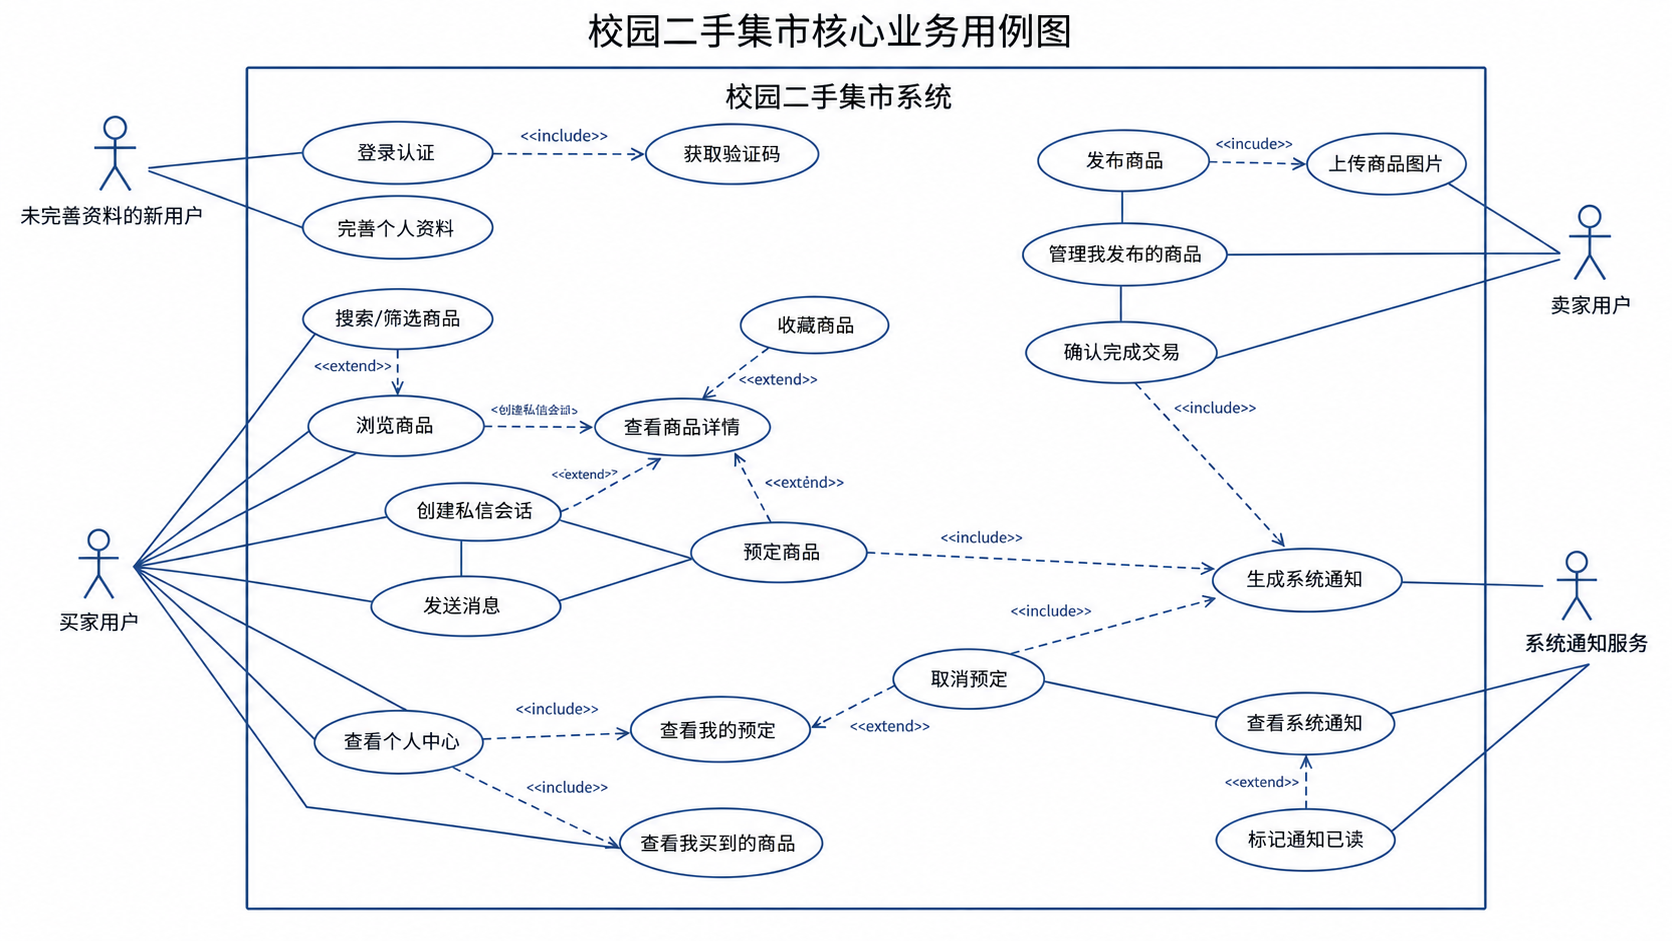
\includegraphics[width=0.95\textwidth]{yongli1.png}
  \caption{校园二手集市核心业务用例图}
  \label{fig:core-use-case}
\end{figure}

\subsection{需求建模图}
需求建模图用于从动态行为和数据流动两个角度补充说明需求。状态机图关注核心业务对象在不同事件触发下如何变化，数据流模型关注外部参与者、处理过程、数据存储和数据流之间的关系。本项目选择商品状态机、订单状态机和数据流模型作为主要需求建模图。

图 \ref{fig:item-state-model} 展示了商品对象的状态变化。商品由卖家发布后进入“在售”状态，买家预定后进入“被预定”状态；若预定取消，商品回到“在售”；若卖家确认交易完成，商品进入“已完成”；若卖家删除或下架商品，则进入“已下架”或逻辑删除状态。该模型对应需求中的商品发布、预定、取消和完成交易流程。

\begin{figure}[H]
  \centering
  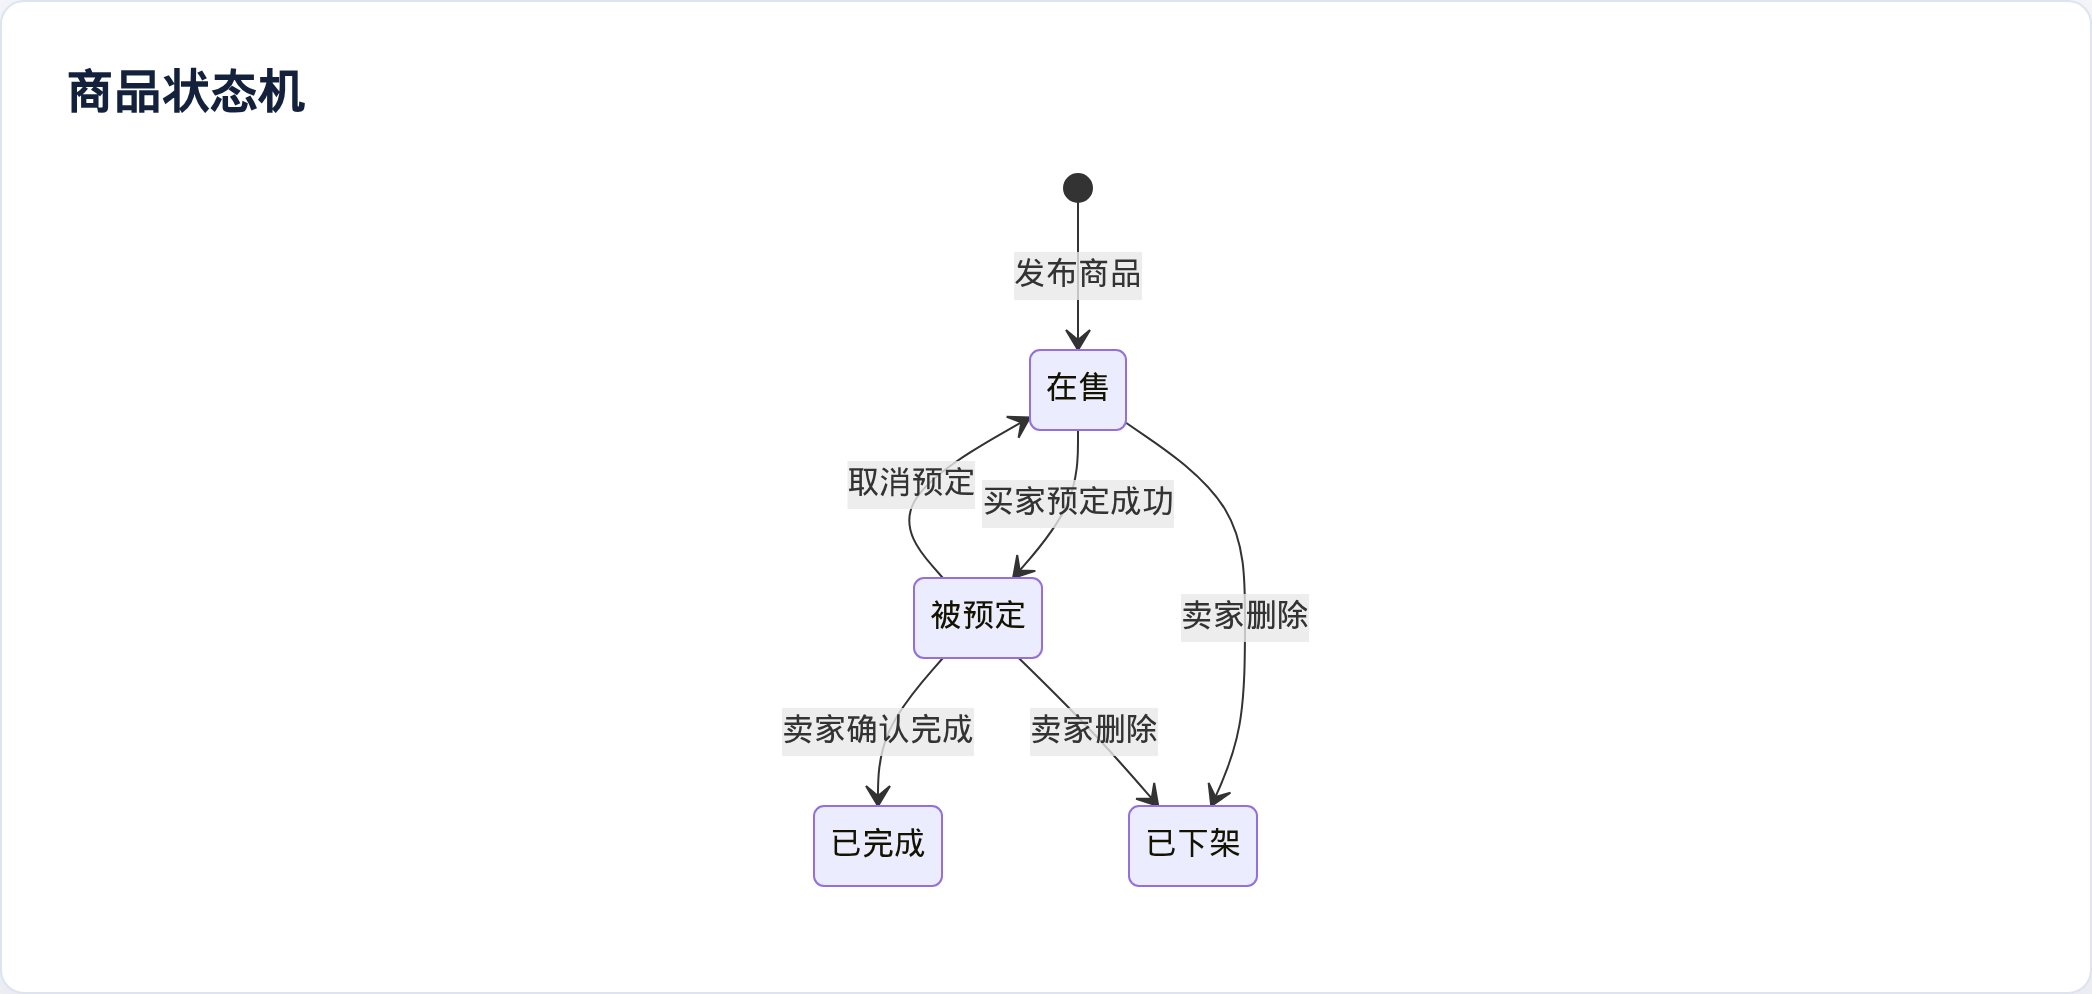
\includegraphics[width=0.8\textwidth]{backend-b-item-state.png}
  \caption{商品状态机图}
  \label{fig:item-state-model}
\end{figure}

图 \ref{fig:order-state-model} 展示了订单对象的状态变化。订单在买家成功预定商品时创建，初始状态为 RESERVED；若交易取消，订单变为 CANCELLED；若卖家确认交易完成，订单变为 COMPLETED。订单状态变化必须与商品状态、会话消息和系统通知保持一致，因此该状态机是交易闭环的关键需求模型。

\begin{figure}[H]
  \centering
  
\includegraphics[width=0.8\textwidth]{backend-b-order-state.png}
  \caption{订单状态机图}
  \label{fig:order-state-model}
\end{figure}

除状态模型外，项目还需要使用数据流模型描述买家、卖家、认证服务、前端页面、后端服务和数据库之间的数据交换。数据流图应体现登录认证、商品发布、商品浏览搜索、私信沟通、交易预定和系统通知等过程，以及用户数据、商品数据、订单数据、消息数据、通知数据和图片文件等数据存储。

\begin{figure}[H]
  \centering
  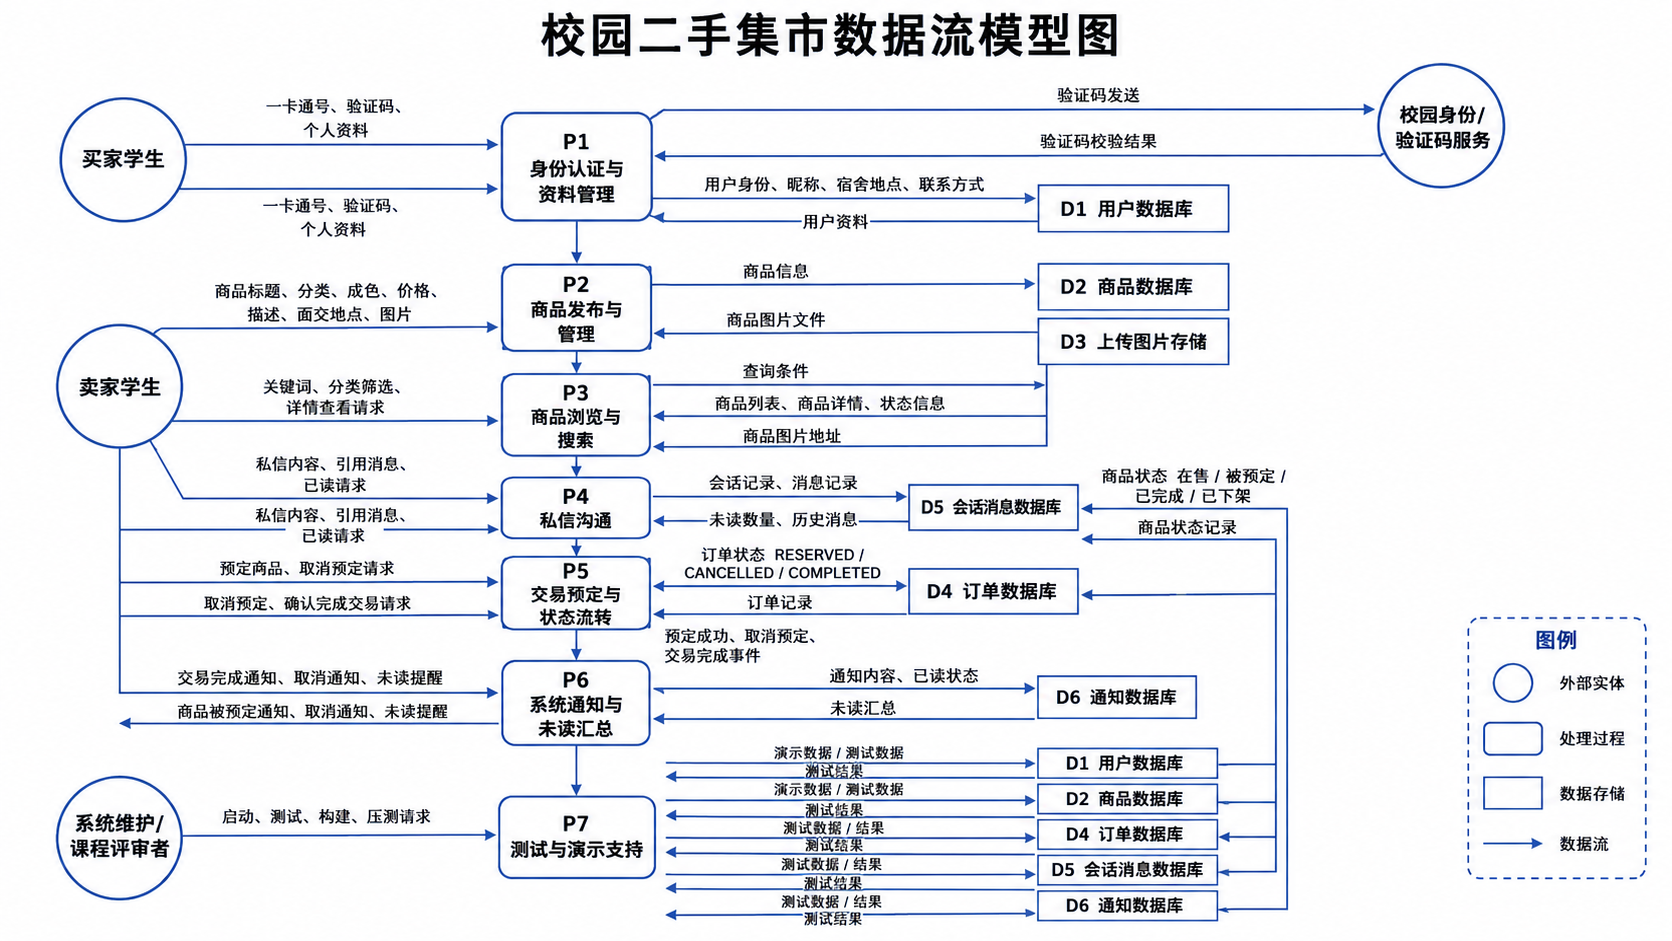
\includegraphics[width=0.95\textwidth]{shujuliu.png}
  \caption{校园二手集市数据流模型图}
  \label{fig:requirement-data-flow}
\end{figure}

\section{用户界面与体验设计}

\subsection{设计目标}
本项目的界面设计采用移动端优先思路，目标用户是在校学生，其主要使用场景是课间、宿舍、食堂或面交前后快速浏览和沟通。因此界面设计强调低学习成本、路径短、反馈明确和状态可见。用户进入系统后应能快速完成登录、浏览、发布、私信、预定和查看个人交易记录等操作，不需要阅读复杂说明。

具体设计目标包括：第一，核心入口固定可见，首页、发布、消息和个人中心通过底部 Tabbar 连接，减少用户寻找功能的成本；第二，商品信息以卡片和详情页方式展示，突出图片、标题、价格、成色、状态和卖家信息；第三，交易状态清晰可见，例如“在售”“被预定”“已完成”等状态标签直接展示在按钮或商品列表中；第四，关键操作提供即时反馈，例如发布、收藏、上传、预定、已读和退出登录都使用 Toast、弹窗或禁用态提示；第五，界面尽量贴近学生熟悉的移动端二手交易体验，使用 Vant 组件提供搜索框、标签页、弹出层、上传组件、图片预览和底部操作栏。

\subsection{页面结构}
系统前端使用 Vue Router 管理页面路由，整体页面结构围绕交易闭环展开。主要页面及职责见表 \ref{tab:page-structure}。

\begin{table}[H]
  \centering
  \caption{主要页面说明}
  \label{tab:page-structure}
  \begin{tabular}{p{3cm}p{3cm}p{7.2cm}}
    \toprule
    页面 & 路由 & 主要职责 \\
    \midrule
    登录页 & \texttt{/login} & 输入一卡通号、获取验证码、完成登录，并根据是否为新用户跳转到新人引导或首页 \\
    新人引导页 & \texttt{/onboarding} & 首次登录后完善昵称、宿舍地点和微信号，使用户具备发布和交易条件 \\
    集市首页 & \texttt{/home} & 展示在售商品瀑布流，支持搜索、分类筛选、下拉刷新和进入详情 \\
    商品详情页 & \texttt{/item/:id} & 展示商品图片、价格、成色、描述、卖家、地点、收藏状态和预定入口 \\
    发布页 & \texttt{/publish} & 上传商品图片，填写标题、分类、成色、价格、地点和描述并发布商品 \\
    消息页 & \texttt{/messages} & 分为私信和系统通知两个标签页，展示未读角标、会话列表和通知列表 \\
    聊天页 & \texttt{/chat/:id} & 展示关联商品和聊天记录，支持发送、引用、撤回和标记已读 \\
    个人中心 & \texttt{/profile} & 展示用户资料、我发布的、我买到的、我的预定、我的收藏和退出登录入口 \\
    \bottomrule
  \end{tabular}
\end{table}

\subsection{原型展示}
本项目在界面设计阶段采用“纸质原型 + 可操作原型”的方式进行验证。纸质原型用于快速确定页面信息层级、底部导航、商品卡片、消息入口和个人中心布局，不追求视觉细节，重点验证用户是否能理解主要操作路径；可操作原型则基于 Vue 3、Vant 和 Tailwind CSS 实现，用于验证页面跳转、表单输入、列表切换和交易状态展示等交互是否可用。

纸质原型主要覆盖首页、商品详情、发布页、消息页和个人中心五类核心页面。小组先在草图中确定移动端页面的基本框架：顶部导航或搜索区位于页面上方，核心内容位于中部，底部使用固定 Tabbar 连接首页、发布、消息和个人中心等高频入口。通过纸质草图，小组能够在编码前快速发现页面入口过多、列表信息密度不足、交易状态不够突出等问题，并在可操作原型中进行调整。

\begin{figure}[H]
  \centering
  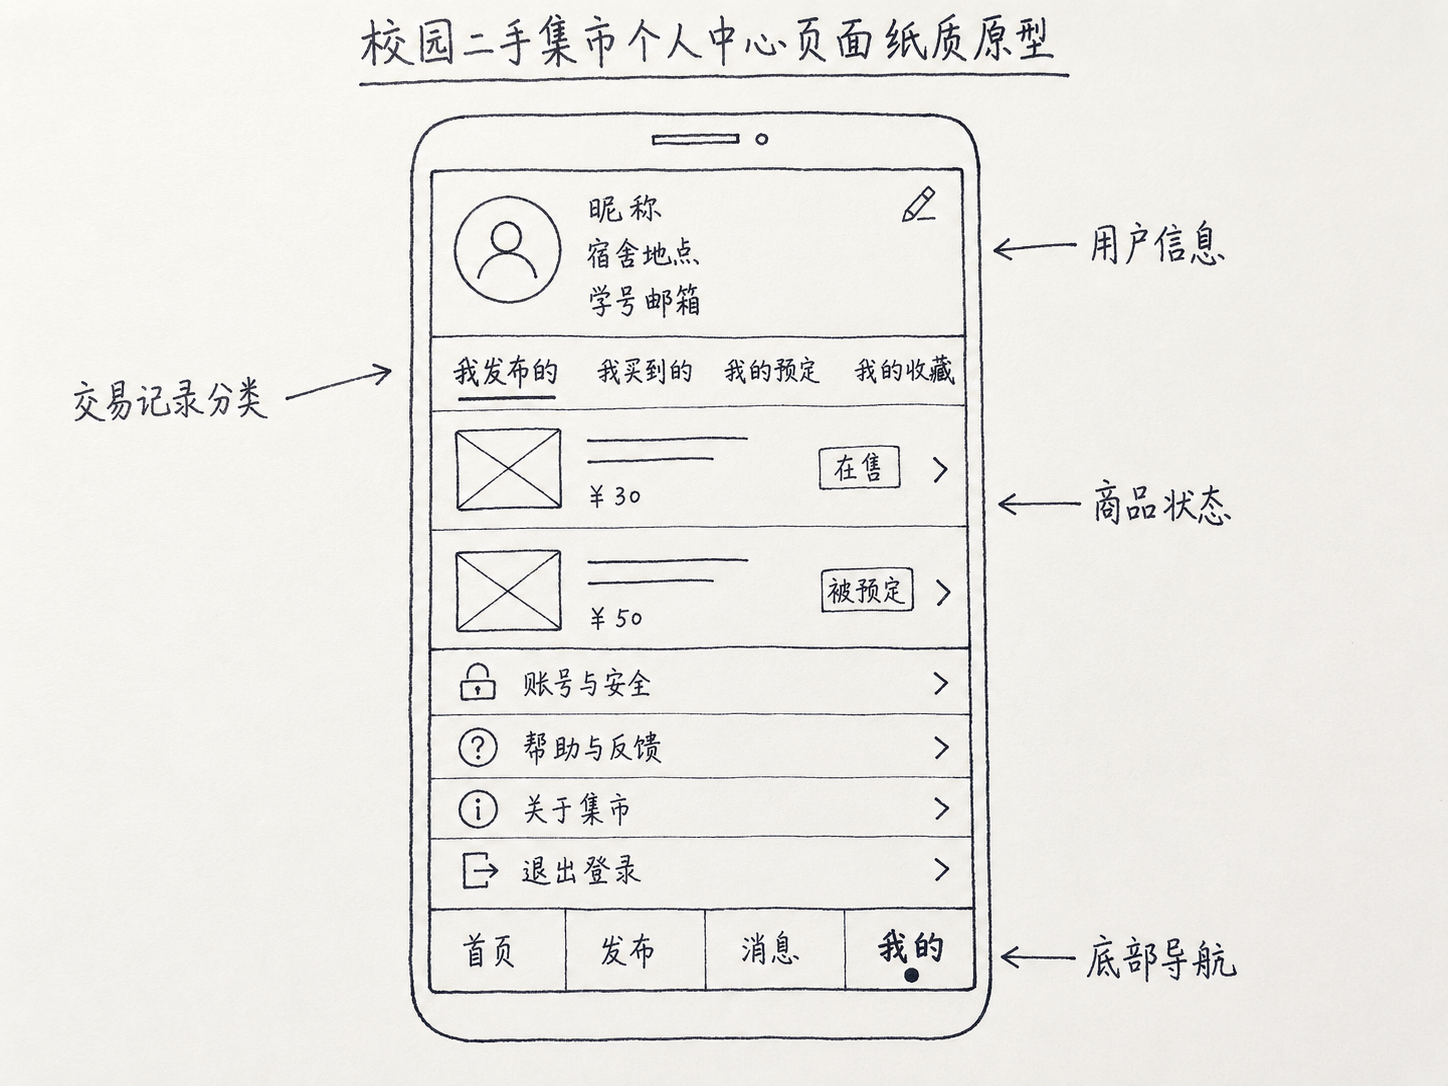
\includegraphics[width=0.85\textwidth]{caotu.png}
  \caption{个人中心纸质快速原型草图}
  \label{fig:paper-prototype-profile}
\end{figure}

在可操作原型中，个人中心页面被实现为一个简易但可交互的页面，如图 \ref{fig:profile-prototype} 所示。页面上方展示用户头像、昵称、常驻地点和学号邮箱；中部通过标签页切换“我发布的”“我买到的”“我的预定”“我的收藏”等列表；下方提供账号与安全、帮助反馈、关于集市和退出登录等入口。该原型用于验证个人交易记录聚合、商品状态标签、资料编辑和退出登录等需求。

\begin{figure}[H]
  \centering
  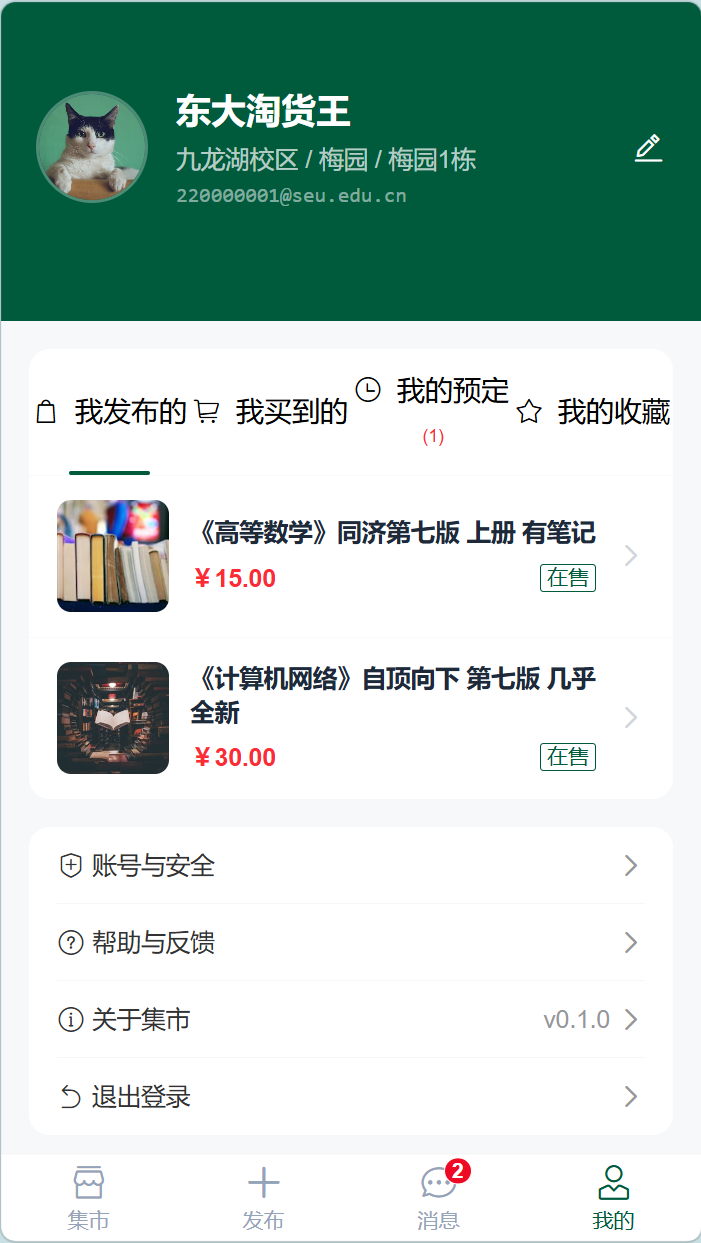
\includegraphics[width=0.35\textwidth]{profile.png}
  \caption{个人中心可操作原型截图}
  \label{fig:profile-prototype}
\end{figure}

\subsection{核心交互流程}
系统核心交互流程围绕“进入平台--发现商品--沟通确认--锁定交易--完成状态流转”展开。

\begin{enumerate}
  \item \textbf{登录与资料完善：}用户打开系统进入登录页，输入 9 位一卡通号并获取验证码，验证码校验通过后获得登录态。若用户资料未完善，系统跳转到新人引导页，要求填写昵称、宿舍地点和微信号；资料保存后进入首页。
  \item \textbf{浏览与搜索商品：}用户进入首页后看到在售商品列表，可以直接浏览，也可以通过搜索框输入关键词，或通过分类标签筛选专业书籍、电子数码、宿舍日用等商品。点击商品卡片后进入详情页。
  \item \textbf{查看详情与收藏：}详情页展示商品图片轮播、价格、成色、标题、描述、浏览量、想要人数、卖家信息和面交地点。用户可以点击收藏按钮保存商品，也可以点击私信或预定入口继续交易流程。
  \item \textbf{发布商品：}卖家进入发布页，上传 1 到 6 张图片，填写标题、分类、成色、价格、地点和描述。系统在前端和后端进行必填项与格式校验，发布成功后跳转到商品详情页。
  \item \textbf{私信沟通：}买家在商品详情页点击私信留言，系统创建或复用围绕该商品的会话。聊天页面展示关联商品卡片和历史消息，用户可以发送文字、引用消息、撤回自己 2 分钟内发送的消息。
  \item \textbf{预定商品：}买家在详情页点击“我想要”，系统弹出确认窗口。确认后后端检查商品是否在售并创建订单，商品状态改为“被预定”，卖家收到系统通知，买家进入聊天页继续约定面交。
  \item \textbf{取消或完成交易：}若交易取消，买家或卖家可取消预定，商品恢复“在售”；若线下面交完成，卖家确认完成交易，订单状态变为 COMPLETED，商品状态变为“已完成”，买家收到完成通知。
  \item \textbf{个人中心查看记录：}用户可在个人中心查看我发布的、我买到的、我的预定和我的收藏，并通过状态标签了解每件商品的当前状态。
\end{enumerate}

\section{系统设计}

\subsection{总体架构}
系统采用前后端分离架构。前端 Vue 应用运行在浏览器中，负责页面渲染、路由跳转、表单输入、图片预览、消息角标和用户交互；后端 Spring Boot 应用提供 REST API，负责认证鉴权、业务规则、事务处理、状态流转和数据持久化。前端通过 \texttt{/api} 调用后端 JSON 接口，通过 \texttt{/uploads} 访问上传图片资源。开发环境中 Vite 代理将这些请求转发到后端 8080 端口。

后端内部采用三层体系结构。表现层由 Controller 组成，负责接收请求、触发参数校验并返回统一 \texttt{Result} 响应；业务逻辑层由 Service 组成，负责用户认证、商品发布、搜索、收藏、交易预定、私信、通知和上传等业务；数据访问层由 Repository 组成，通过 Spring Data JPA 访问数据库。实体对象位于 Entity 层，用于描述用户、商品、订单、会话、消息和通知等业务概念。开发和测试环境默认使用 H2 内存数据库，后续部署可通过 MySQL profile 切换到 MySQL。

\subsection{系统设计图}
本项目的总体架构采用“客户端/服务器风格 + 三层体系结构风格”。从外部通信看，浏览器端 Vue 应用作为客户端，通过 HTTP/JSON 请求访问 Spring Boot 后端服务，后端作为服务器统一提供认证、用户、商品、交易、消息、通知和上传等 REST API。从后端内部组织看，系统进一步划分为表现层、业务逻辑层和数据访问与存储层：表现层由各类 Controller、统一响应和全局异常处理组成；业务逻辑层由 Service 组件实现权限校验、交易规则、状态流转、通知生成和文件上传逻辑；数据访问层通过 Spring Data JPA Repository 访问 H2/MySQL 数据库，并通过上传目录保存商品图片。

选择该架构的原因主要有三点。第一，前后端分离使界面开发和后端接口开发可以并行推进，符合课程项目周期较短、成员分工明确的特点。第二，三层体系结构能够将用户界面、业务规则和数据持久化解耦，降低代码修改影响范围，例如商品状态规则变化时主要修改业务逻辑层，不需要重写前端页面或数据库访问方式。第三，Repository 访问层使系统可以在开发演示阶段使用 H2 数据库，在后续部署阶段切换到 MySQL，提升便携性和可维护性。

\begin{figure}[H]
  \centering
  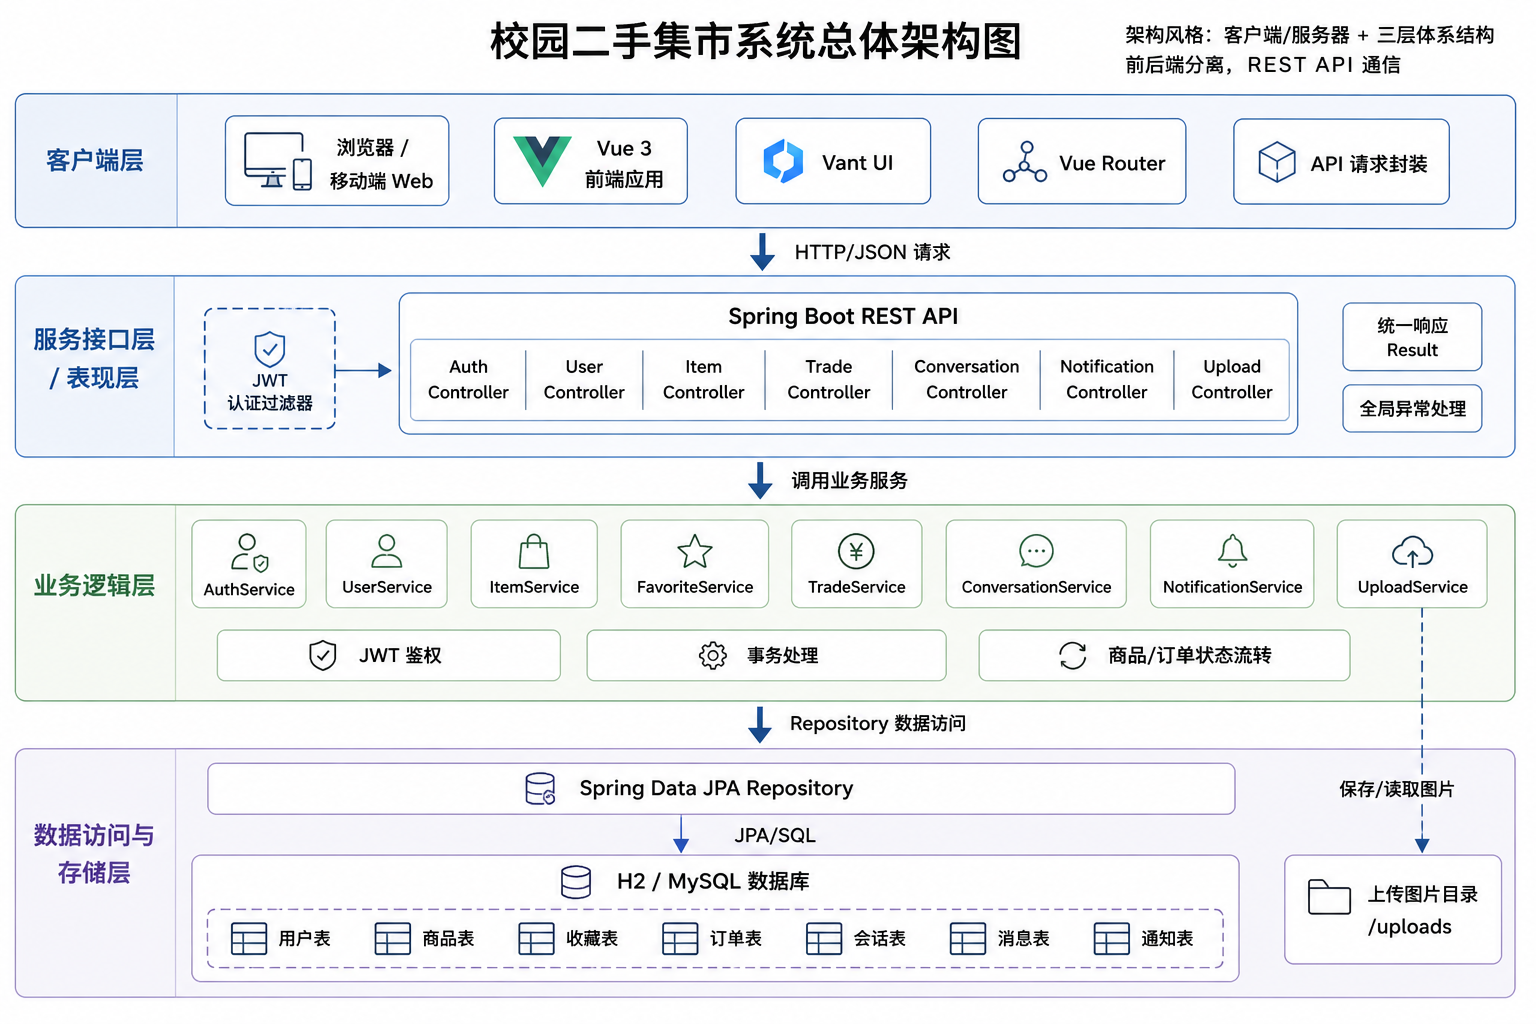
\includegraphics[width=0.95\textwidth]{xitongsheji.png}
  \caption{系统总体架构图}
  \label{fig:system-architecture}
\end{figure}

如图 \ref{fig:system-architecture} 所示，客户端层负责页面展示、路由跳转和用户交互；服务接口层负责接收请求、执行认证鉴权、参数校验和统一响应；业务逻辑层负责实现校园二手交易的核心规则，包括商品发布、浏览搜索、私信会话、预定锁定、取消预定、确认完成和系统通知；数据访问与存储层负责持久化用户、商品、收藏、订单、会话、消息和通知等数据。该设计既体现了客户端/服务器架构的通信关系，也体现了三层体系结构中各层之间单向依赖、职责清晰的设计原则。

\subsection{组件图}
组件图从逻辑模块角度展示系统的组成和接口依赖关系，如图 \ref{fig:component-diagram} 所示。前端 Vue 应用通过 REST API 调用后端接口组件，后端接口组件包括认证、用户、商品、交易、消息、通知和上传等 API。每个接口组件向前端提供明确的服务接口，同时依赖对应的业务服务完成具体逻辑。业务服务层通过 JPA Repository 访问数据库，并由上传服务读写商品图片文件。

在组件关系上，认证服务依赖验证码或校园身份验证能力；商品服务依赖商品、图片、地点和用户数据；交易服务除依赖订单和商品数据外，还需要调用会话消息服务和通知服务，在预定、取消和完成交易时同步创建会话或生成系统通知。通过这种组件划分，系统能够将界面交互、接口暴露、业务规则和数据访问分离，便于后续扩展管理员后台、举报审核或 WebSocket 消息推送等功能。

\begin{figure}[H]
  \centering
  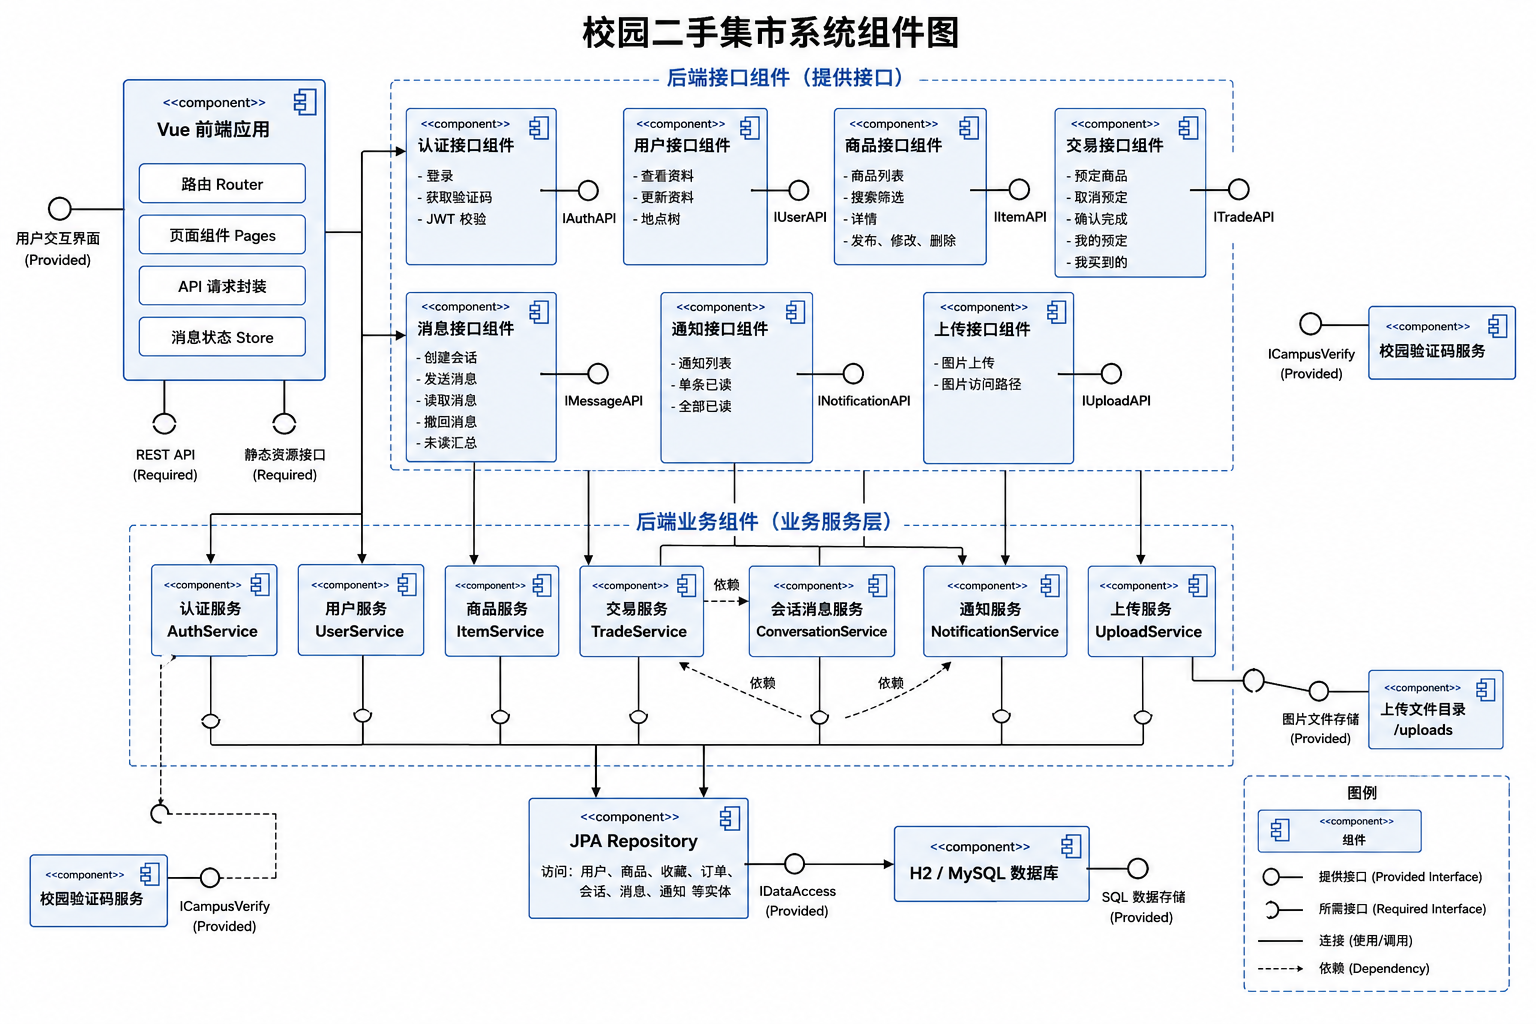
\includegraphics[width=0.95\textwidth]{zujiantu.png}
  \caption{系统组件图}
  \label{fig:component-diagram}
\end{figure}

\subsection{部署图}
部署图从运行环境角度展示系统的物理节点、部署产物和通信关系，如图 \ref{fig:deployment-diagram} 所示。用户通过手机或 PC 浏览器访问前端页面；前端静态资源在开发阶段由 Vite Dev Server 提供，在后续部署阶段可由 Nginx 或其他静态资源服务器提供。浏览器通过 HTTP/JSON 调用 Spring Boot 后端 API，开发环境中也可以通过 Vite 代理将 \texttt{/api} 和 \texttt{/uploads} 请求转发到后端。

后端应用运行在 Java 17 和 Spring Boot 环境中，对外提供 8080 端口服务。数据库在课程演示阶段默认使用 H2 内存数据库，便于快速启动和自动初始化；若切换到部署环境，可通过 MySQL profile 使用 MySQL 数据库。上传图片存储在 \texttt{uploads} 目录中，由后端上传服务负责写入和读取。验证码服务在开发阶段由固定验证码模拟，正式环境可替换为校园邮箱或统一身份认证接口。

\begin{figure}[H]
  \centering
  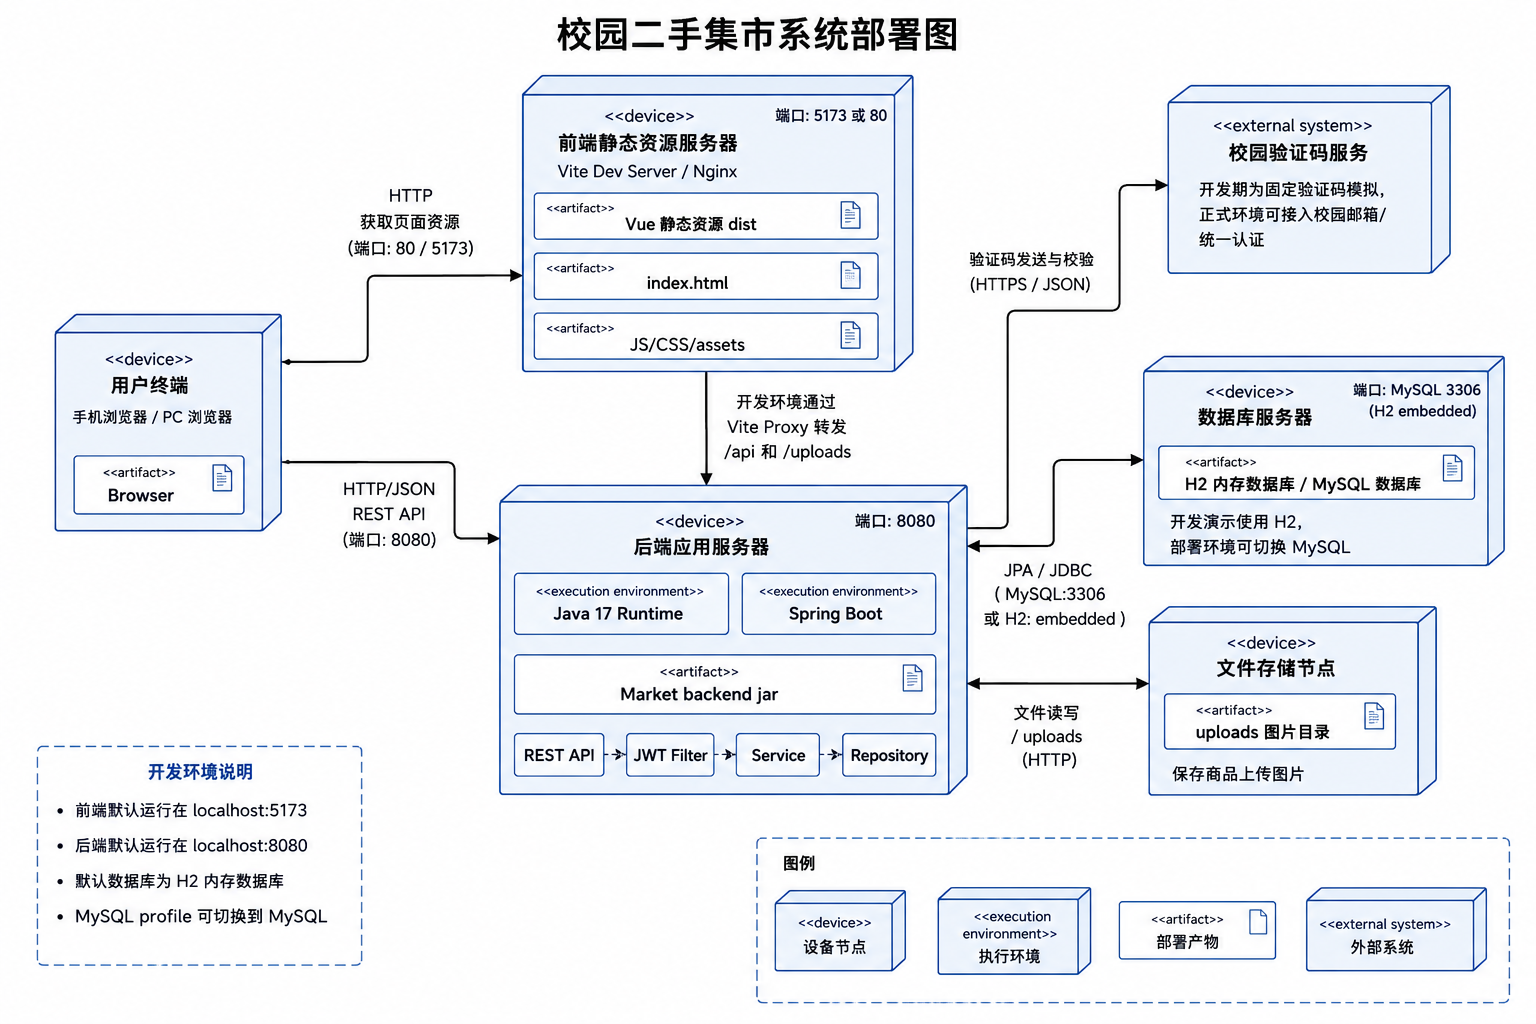
\includegraphics[width=0.95\textwidth]{bushutu.png}
  \caption{系统部署图}
  \label{fig:deployment-diagram}
\end{figure}

\subsection{数据库设计}
数据库设计围绕用户、商品、交易、消息和通知五类核心数据展开。系统使用 JPA 自动维护实体映射，同时保留 \texttt{backend/src/main/resources/db/schema.sql} 作为表结构参考。图 \ref{fig:database-er} 展示了交易、消息和通知相关实体之间的主要关系。

\begin{figure}[H]
  \centering
  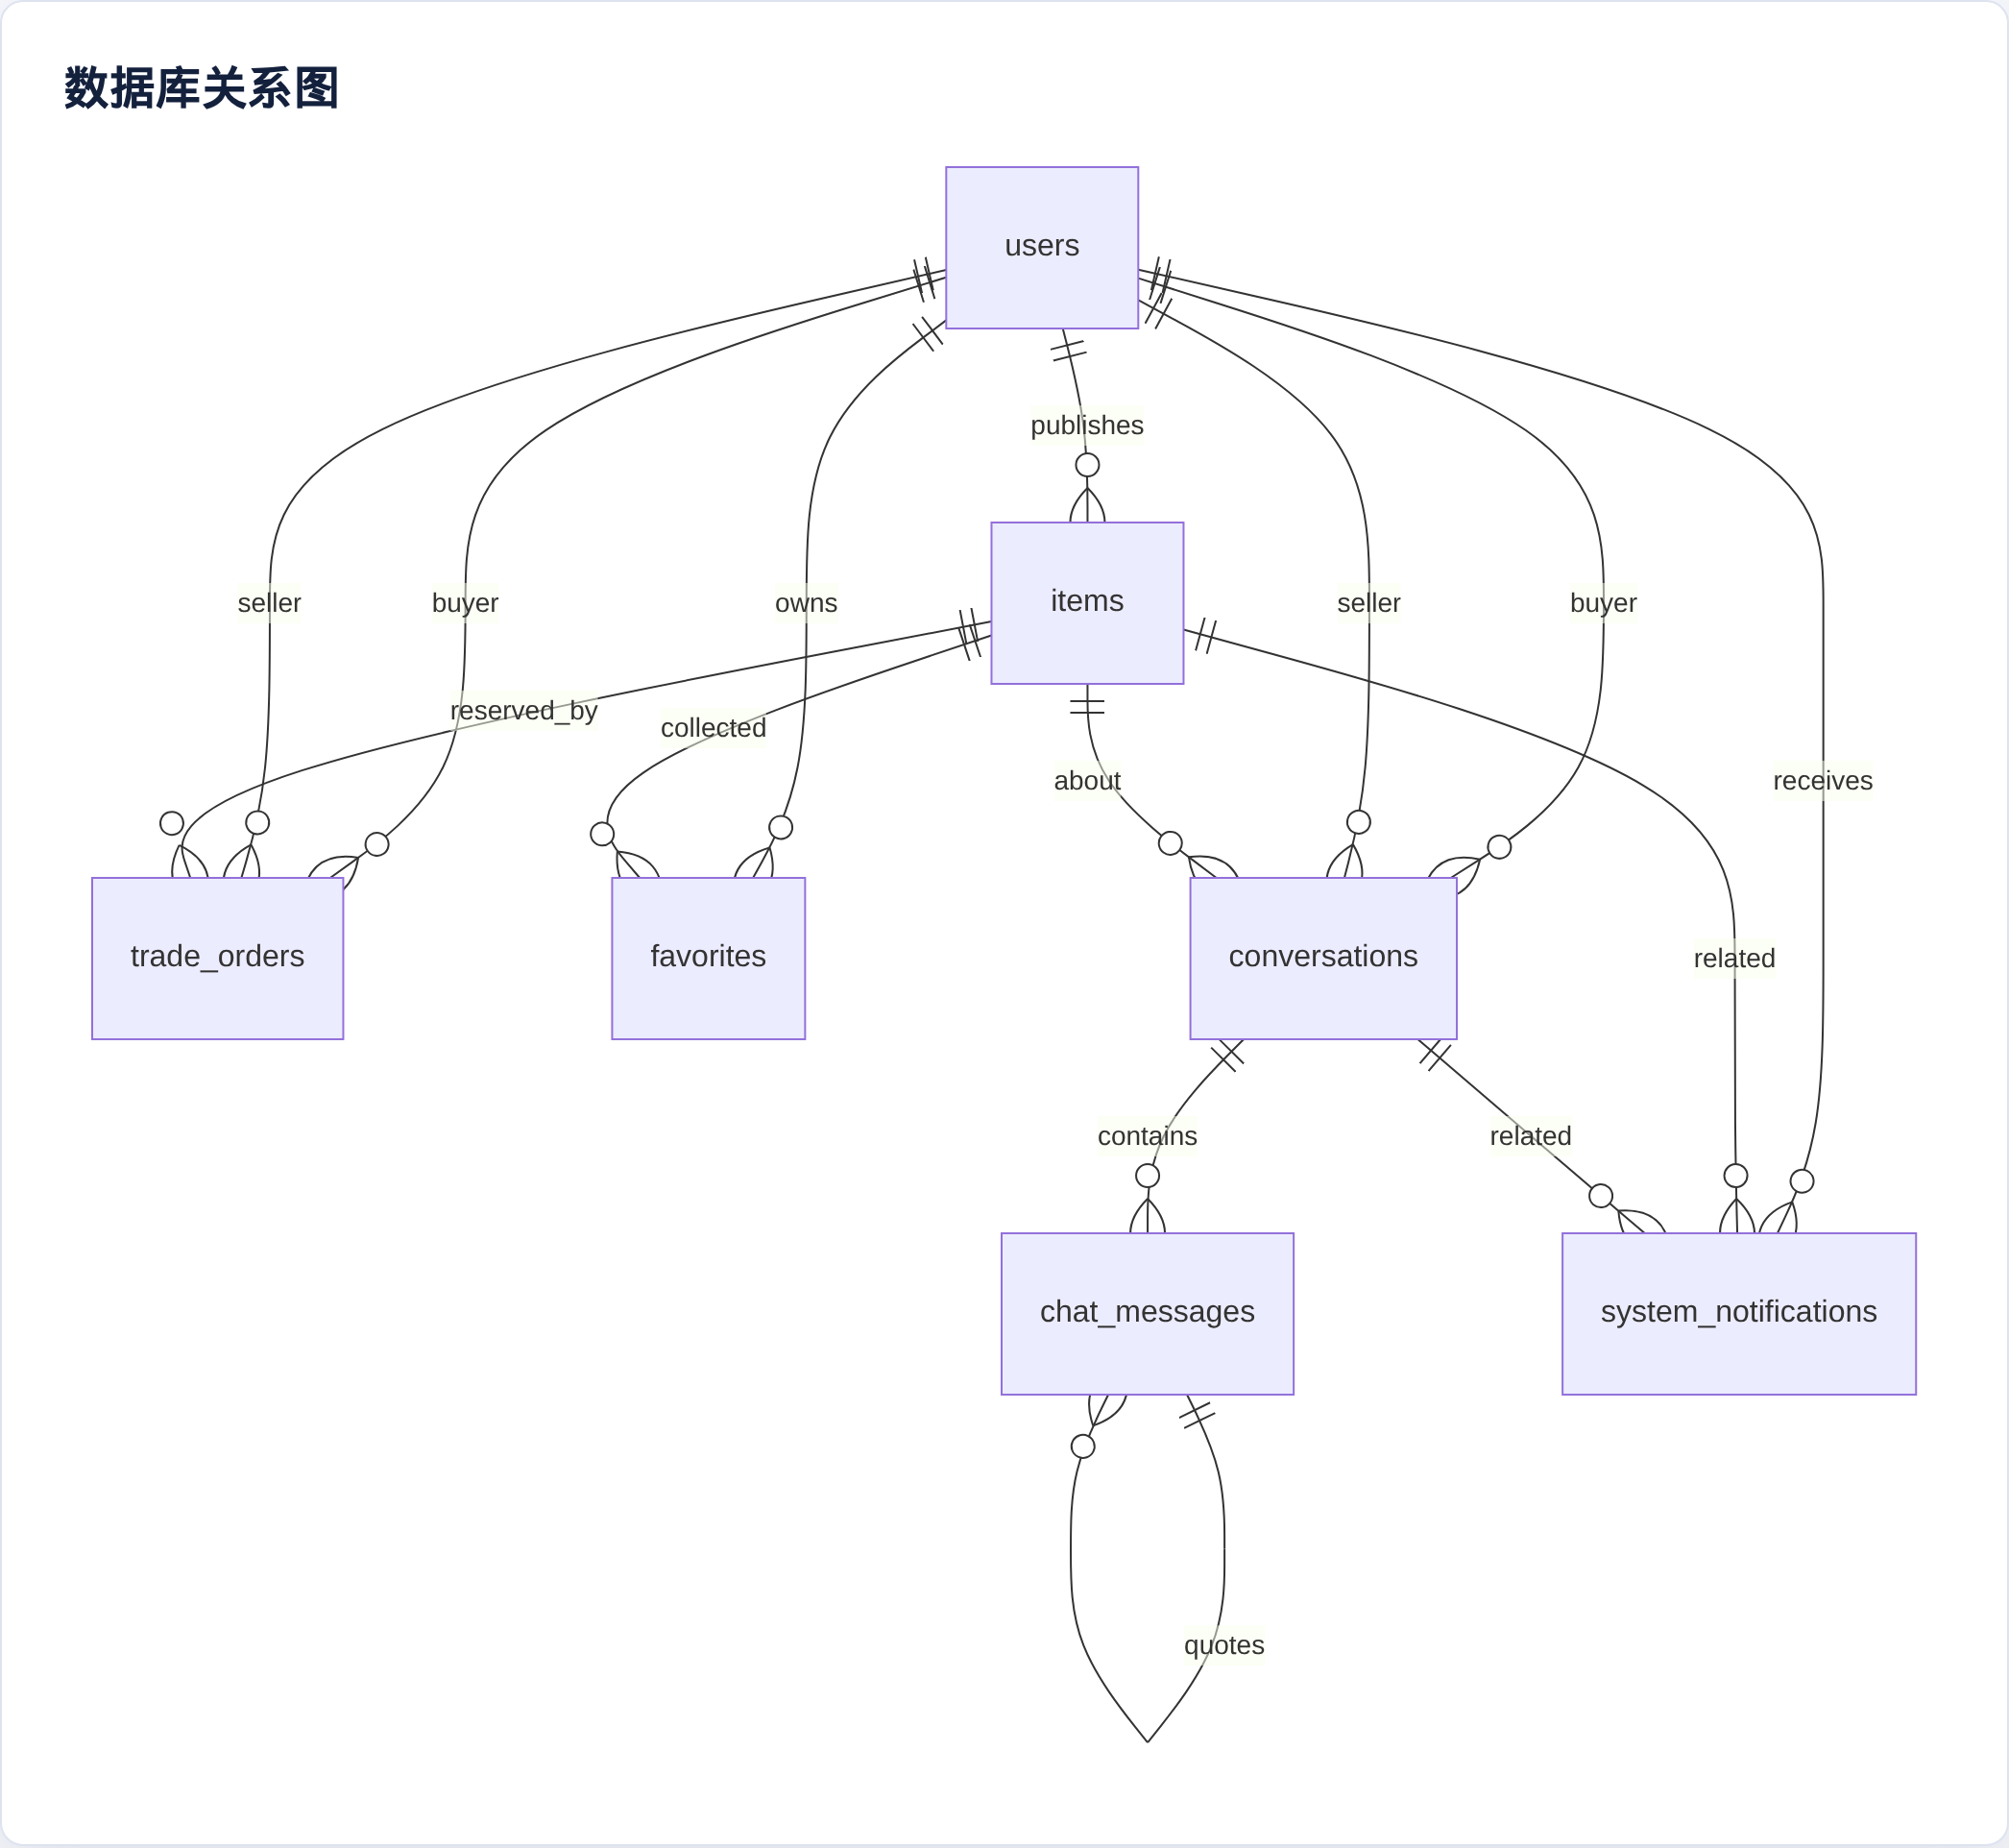
\includegraphics[width=0.9\textwidth]{backend-b-er.png}
  \caption{数据库核心实体关系图}
  \label{fig:database-er}
\end{figure}

数据库中，\texttt{users} 表保存学生身份、昵称、头像、微信号和常驻地点；\texttt{location} 表以父子关系保存校区、苑区和楼栋；\texttt{items} 表保存商品标题、价格、成色、分类、描述、封面图、状态、想要人数和浏览量；\texttt{item\_images} 表保存商品多图；\texttt{favorites} 表保存用户收藏商品的多对多关系；\texttt{trade\_orders} 表保存商品预定、取消和完成状态；\texttt{conversations} 和 \texttt{chat\_messages} 表保存围绕商品形成的私信会话和消息记录；\texttt{system\_notifications} 表保存预定、取消和完成交易等系统通知。

\begin{table}[H]
  \centering
  \caption{核心数据表说明}
  \small
  \setlength{\tabcolsep}{3pt}
  \renewcommand{\arraystretch}{1.18}
  \begin{tabular}{L{3.1cm}L{5.6cm}L{5.2cm}}
    \toprule
    数据表 & 主要字段 & 说明 \\
    \midrule
    \texttt{users} & student\_id、email、nickname、wechat、location\_id、is\_profile\_complete & 平台用户和资料完成状态 \\
    \texttt{location} & parent\_id、name、code、level & 校区/苑区/楼栋树形地点数据 \\
    \texttt{items} & seller\_id、location\_id、title、price、category、status、is\_deleted & 商品主体信息和状态 \\
    \texttt{item\_images} & item\_id、url、sort\_order & 商品图片列表和展示顺序 \\
    \texttt{favorites} & user\_id、item\_id & 用户收藏关系，限制同一用户重复收藏同一商品 \\
    \texttt{trade\_orders} & item\_id、buyer\_id、seller\_id、status、cancelled\_at、completed\_at & 订单状态流转记录 \\
    \texttt{conversations} & item\_id、buyer\_id、seller\_id、last\_message、unread\_count & 买卖双方围绕商品形成的会话 \\
    \texttt{chat\_messages} & conversation\_id、sender\_id、recipient\_id、content、quote\_message\_id、recalled & 私信消息、引用和撤回状态 \\
    \shortstack[l]{\texttt{system\_}\\\texttt{notifications}} & user\_id、type、title、content、item\_id、conversation\_id、is\_read & 系统通知和已读状态 \\
    \bottomrule
  \end{tabular}
\end{table}

在关系约束方面，一个用户可以发布多个商品，一个商品属于一个卖家；一个商品可以有多张图片；收藏表通过用户和商品形成唯一约束；订单同时关联商品、买家和卖家；会话通过商品、买家和卖家唯一确定，避免同一买家围绕同一商品重复创建多个会话；消息属于会话，并可引用同一会话中的另一条消息；通知属于接收用户，并可关联商品和会话。

\subsection{接口设计}
后端接口采用 REST 风格设计，统一以 \texttt{/api} 为前缀，使用 JSON 作为请求和响应格式。成功响应统一返回 \texttt{code=0}，业务失败返回对应错误码和错误信息。主要接口按认证、用户、商品、收藏、交易、消息、通知和上传分类，见表 \ref{tab:main-apis}。

\begingroup
\small
\setlength{\tabcolsep}{3pt}
\renewcommand{\arraystretch}{1.18}
\begin{longtable}{L{5.0cm}L{2.3cm}L{6.3cm}}
  \caption{主要接口说明}\label{tab:main-apis} \\
  \toprule
  接口 & 方法 & 功能说明 \\
  \midrule
  \endfirsthead
  \toprule
  接口 & 方法 & 功能说明 \\
  \midrule
  \endhead
  \path|/api/auth/send-code| & POST & 根据一卡通号发送或生成验证码 \\
  \path|/api/auth/login| & POST & 校验验证码，返回 JWT、用户 id 和是否新用户 \\
  \path|/api/users/me| & GET/PUT & 获取或更新当前用户资料 \\
  \path|/api/locations/tree| & GET & 获取校区、苑区、楼栋级联地点树 \\
  \path|/api/items| & GET/POST & 查询商品列表或发布新商品，支持分类、关键词和状态筛选 \\
  \path|/api/items/mine| & GET & 查询当前用户发布的商品 \\
  \path|/api/items/{id}| & \shortstack[l]{GET/PUT/\\DELETE} & 查看、修改或删除指定商品 \\
  \path|/api/upload/image| & POST & 上传商品图片，返回 \path|/uploads/| 访问路径 \\
  \path|/api/items/{id}/favorite| & \shortstack[l]{POST/\\DELETE} & 收藏或取消收藏指定商品 \\
  \path|/api/favorites| & GET & 查询当前用户收藏列表 \\
  \path|/api/items/{id}/reserve| & POST & 买家预定在售商品，创建订单和会话 \\
  \path|/api/orders/{id}/cancel| & POST & 买家或卖家取消预定订单 \\
  \path|/api/orders/{id}/complete| & POST & 卖家确认交易完成 \\
  \path|/api/orders/reserved| & GET & 查询当前买家的预定商品 \\
  \path|/api/orders/bought| & GET & 查询当前买家已完成购买的商品 \\
  \path|/api/conversations| & GET/POST & 查询会话列表或创建商品会话 \\
  \path|/api/conversations/{id}/messages| & GET/POST & 查询会话消息或发送消息 \\
  \path|/api/conversations/{id}/read| & POST & 将指定会话标记为已读 \\
  \path|/api/messages/{id}/recall| & POST & 撤回 2 分钟内自己发送的消息 \\
  \path|/api/messages/unread-summary| & GET & 获取私信、通知和总未读数 \\
  \path|/api/notifications| & GET & 查询系统通知列表 \\
  \path|/api/notifications/{id}/read| & POST & 将指定通知标记为已读 \\
  \path|/api/notifications/read-all| & POST & 将当前用户通知全部标记为已读 \\
  \path|/api/health| & GET & 后端健康检查 \\
  \bottomrule
\end{longtable}
\endgroup

\subsection{安全机制}
本项目虽然是课程实验系统，但仍围绕校园二手交易的核心风险设计了基础安全机制。系统需要保护用户身份、个人资料、商品操作权限、订单状态和聊天内容，避免未登录访问、越权修改、一物多卖、非法文件上传和异常信息泄露等问题。后端安全机制主要由 Spring Security、JWT、统一异常处理、参数校验、文件上传限制和事务控制共同组成。

\subsubsection{认证与会话管理}
系统采用基于 JWT 的无状态认证方式。用户通过一卡通号和验证码完成登录后，后端生成包含用户 id 和一卡通号的 JWT，并由前端保存在本地。后续请求通过 \texttt{Authorization: Bearer token} 头携带令牌，后端的 \texttt{JwtAuthFilter} 在请求进入 Controller 前校验令牌合法性；校验通过后，将用户 id 写入 \texttt{UserContext} 和 Spring Security 上下文，供后续业务方法识别当前用户。

后端配置为无状态会话模式，不依赖服务器端 Session 存储登录状态。这种方式适合前后端分离系统，便于后续横向扩展和前端独立部署。系统只放行 \texttt{/api/auth/**}、\texttt{/api/health} 和 \texttt{/uploads/**} 等公开接口，其余 \texttt{/api/**} 接口都要求已认证访问。未登录访问会返回 401 和“请先登录”，已登录但无权限访问会返回 403 和“无权访问”。

\subsubsection{开发期认证开关}
为便于课程演示和接口测试，系统提供了开发期认证 Header：当 \texttt{app.security.dev-auth-enabled=true} 时，后端允许通过 \texttt{X-Dev-User-Id} 指定当前用户。这一机制降低了 MockMvc 测试和本地联调成本。正式或 MySQL profile 中应关闭该开关，即 \texttt{app.security.dev-auth-enabled=false}，避免绕过 JWT 登录流程。报告和维护说明中需要明确：开发期 Header 只能用于本地演示和测试环境，不能在生产环境开启。

\subsubsection{权限控制与越权防护}
系统在 Service 层进行细粒度权限校验。商品修改和删除只能由商品卖家执行；订单取消只能由买家或卖家执行；确认交易完成只能由卖家执行；私信会话和消息只能由会话参与者查看和操作；用户不能预定自己发布的商品。相比只在前端隐藏按钮，后端校验能够防止用户直接构造 HTTP 请求绕过界面限制。

交易相关操作还会检查业务状态。例如只有“在售”商品可以被预定，只有 RESERVED 状态订单可以取消或完成，已完成商品不能再次预定。商品预定、取消和完成交易都放在事务中执行，并对关键商品或订单记录使用悲观锁，降低并发请求造成一物多卖或状态不一致的风险。

\subsubsection{输入校验与数据约束}
后端 DTO 使用 Bean Validation 对用户输入进行约束。例如一卡通号必须为 9 位数字，验证码必须符合长度和数字格式；商品标题不能为空且不超过 40 个字符，描述不超过 500 个字符，价格必须大于等于 0.01，图片数量最多 6 张；聊天消息不能为空且不超过 200 个字符；用户昵称、微信号、头像地址也有长度限制。Controller 使用 \texttt{@Valid} 触发校验，校验失败时由统一异常处理返回明确的业务错误信息。

这些限制既提升了用户体验，也降低了异常数据进入数据库的概率。对商品地点，系统要求使用地点树中已有的 \texttt{locationCode}，避免用户随意填写不可识别地点。对交易状态，系统使用固定状态值描述商品和订单流转，便于前端展示、后端校验和测试覆盖。

\subsubsection{文件上传安全}
商品图片上传是系统中较容易产生安全风险的入口。后端上传服务对文件进行了多重限制：文件不能为空，单个文件大小不能超过 5MB，\texttt{Content-Type} 必须以 \texttt{image/} 开头，扩展名只允许 \texttt{jpg}、\texttt{jpeg}、\texttt{png}、\texttt{gif} 和 \texttt{webp}。保存文件时系统使用 UUID 生成新文件名，避免直接使用用户上传的原始文件名；同时对目标路径进行 normalize 和根目录校验，防止路径穿越。

上传成功后，系统只返回 \texttt{/uploads/} 下的访问路径。开发环境中该目录用于本地演示，后续若进入正式部署，可将其迁移到独立对象存储或受控静态资源服务，并增加图片压缩、病毒扫描和访问频率限制等增强措施。

\subsubsection{统一异常与响应格式}
系统使用统一响应结构 \texttt{Result} 返回数据，成功时 \texttt{code=0}，失败时返回业务错误码和错误信息。业务异常、参数校验异常、上传大小异常和未知异常由 \texttt{GlobalExceptionHandler} 集中处理。这样可以避免后端异常堆栈直接暴露给前端用户，同时让前端能够按照统一格式展示 Toast、空状态和错误提示。

对认证和授权异常，系统使用专门的 \texttt{ApiAuthenticationEntryPoint} 和 \texttt{ApiAccessDeniedHandler} 返回 JSON 格式错误，而不是跳转到默认登录页。这一点对于前后端分离系统很重要，因为前端需要接收结构化错误后自行决定是否跳转登录页或展示无权限提示。

\subsubsection{跨域与接口访问控制}
前端开发服务器和后端服务运行在不同端口，因此系统配置了 CORS。当前开发期允许 \texttt{localhost} 和 \texttt{127.0.0.1} 的多端口来源，支持常用 HTTP 方法和请求头，并允许携带认证信息。该设置满足 Vite 开发服务器端口变化和本地联调需要。若进入正式部署，应将允许来源收紧为实际域名，避免任意站点跨域调用 API。

\subsubsection{安全机制小结}
表 \ref{tab:security-mechanisms} 总结了本项目采用的主要安全机制及其对应风险。

\begin{table}[H]
  \centering
  \caption{安全机制与风险控制}
  \label{tab:security-mechanisms}
  \begin{tabular}{p{3.2cm}p{4.4cm}p{5.8cm}}
    \toprule
    安全机制 & 主要防护目标 & 实现方式 \\
    \midrule
    JWT 认证 & 防止未登录用户访问受保护接口 & 登录后生成 JWT，请求通过 Bearer Token 携带，过滤器统一校验 \\
    Spring Security 鉴权 & 区分公开接口与受保护接口 & 公开认证、健康检查和上传访问接口，其余 \texttt{/api/**} 需要认证 \\
    Service 层权限校验 & 防止越权修改商品、订单和会话 & 商品、订单、会话和消息操作均检查当前用户是否为合法参与者 \\
    事务与悲观锁 & 防止并发预定导致一物多卖 & 预定、取消、完成交易在事务内执行，并锁定关键商品或订单记录 \\
    参数校验 & 防止非法输入进入业务逻辑和数据库 & 使用 Bean Validation 限制学号、验证码、标题、价格、消息长度等字段 \\
    文件上传限制 & 防止非法文件、超大文件和路径穿越 & 校验文件类型、扩展名和大小，使用 UUID 文件名并检查保存路径 \\
    统一异常处理 & 防止异常信息泄露并统一前端处理 & 使用 \texttt{Result}、全局异常处理器和认证/授权错误处理器返回 JSON 错误 \\
    CORS 配置 & 支持本地联调并限制跨域来源 & 开发期允许 localhost 多端口，正式部署时应收紧为指定域名 \\
    开发期认证开关 & 平衡测试便利性和正式环境安全 & \texttt{X-Dev-User-Id} 仅在开发配置开启，正式 profile 中关闭 \\
    \bottomrule
  \end{tabular}
\end{table}

总体而言，本项目的安全设计以课程项目可实现范围为边界，重点覆盖身份认证、权限控制、输入校验、上传安全和交易一致性。对于正式生产环境，还需要进一步补充 HTTPS、真实校园统一身份认证、日志审计、敏感信息脱敏、上传文件安全扫描、访问频率限制和数据库备份策略。

\section{程序开发}

\subsection{代码组织}
项目采用前后端分离的代码组织方式。后端位于 \texttt{backend/} 目录，使用 Spring Boot 构建 REST API；前端位于 \texttt{frontend/} 目录，使用 Vue 3、Vite、Vant 和 Tailwind CSS 构建移动端 Web 页面；文档和报告素材位于 \texttt{docs/} 目录，测试和报告辅助脚本位于 \texttt{scripts/} 目录。这样的组织方式使页面开发、接口开发、测试文档和报告材料相互独立，便于小组成员并行工作。

后端代码主包为 \texttt{Market\_backend}，整体采用分层结构。Controller 层负责暴露 HTTP 接口和接收请求参数，Service 层负责业务规则和事务处理，Repository 层负责数据库访问，Entity 层负责持久化对象建模，DTO 层负责前后端数据传输，Config 和 Common 层提供安全、跨域、JWT、统一响应和异常处理等公共能力。前端代码则按页面组件、接口封装和状态管理组织：页面组件负责具体视图，\texttt{api/} 目录封装后端请求，\texttt{stores/} 目录保存消息和未读状态等跨页面状态。

\begin{table}[H]
  \centering
  \caption{项目代码组织}
  \small
  \setlength{\tabcolsep}{3pt}
  \renewcommand{\arraystretch}{1.18}
  \begin{tabular}{L{5.0cm}L{3.8cm}L{5.1cm}}
    \toprule
    目录或包 & 主要内容 & 职责说明 \\
    \midrule
    \path|backend/src/main/java/Market_backend/controller| & AuthController、ItemController、TradeController 等 & 接收 HTTP 请求，调用 Service，返回统一响应结果 \\
    \path|backend/src/main/java/Market_backend/service| & AuthService、ItemService、TradeService、ConversationService 等 & 实现认证、商品、交易、消息、通知、上传等核心业务逻辑 \\
    \path|backend/src/main/java/Market_backend/repository| & UserRepository、ItemRepository、TradeOrderRepository 等 & 基于 Spring Data JPA 完成实体查询、保存和悲观锁查询 \\
    \path|backend/src/main/java/Market_backend/entity| & User、Item、TradeOrder、Conversation 等 & 对应数据库核心表，描述业务对象及其关联关系 \\
    \path|backend/src/main/java/Market_backend/dto| & Request 和 VO 对象 & 接收前端请求参数，返回页面需要的数据结构，并承载参数校验规则 \\
    \path|backend/src/main/java/Market_backend/config| & SecurityConfig、JwtAuthFilter、CorsConfig 等 & 配置认证鉴权、JWT、跨域、静态资源和初始化数据 \\
    \path|backend/src/main/java/Market_backend/common| & Result、BusinessException、UserContext 等 & 提供统一响应、业务异常和当前用户上下文 \\
    \path|frontend/src/components| & Login、Home、Detail、Publish、Messages、Chat、Profile 等 & 实现主要页面和可交互视图 \\
    \path|frontend/src/api| & auth、items、trade、messages、upload 等请求封装 & 统一调用后端 REST API，处理 Token 和错误响应 \\
    \path|frontend/src/stores| & messages 状态逻辑 & 保存私信、通知、未读角标和聊天元数据 \\
    \bottomrule
  \end{tabular}
\end{table}

从模块划分看，后端以业务领域进行组织，而不是按页面组织。认证、用户、商品、收藏、交易、消息、通知和上传分别形成独立的 Controller、Service、Repository 或 DTO 组合。前端虽然以页面为中心，但所有网络请求都集中到 \texttt{api/} 目录，避免在页面组件中直接拼接请求逻辑。这样既保持了页面代码的可读性，也便于接口路径或认证方式变化时集中修改。

\subsection{面向对象设计}
后端面向对象设计围绕校园二手交易中的核心概念展开。系统抽象出的主要对象包括用户、地点、商品、商品图片、收藏、交易订单、会话、聊天消息和系统通知。这些对象既对应现实业务中的名词，也对应数据库中的持久化实体。对象之间通过一对多、多对一和唯一约束关系连接，形成从“用户发布商品”到“买家预定商品”再到“双方沟通并完成交易”的完整对象网络。

核心对象及关系如表 \ref{tab:object-model} 所示。

\begin{table}[H]
  \centering
  \caption{核心对象抽象与关系}
  \label{tab:object-model}
  \small
  \setlength{\tabcolsep}{3pt}
  \renewcommand{\arraystretch}{1.18}
  \begin{tabular}{L{3.4cm}L{4.2cm}L{6.3cm}}
    \toprule
    对象 & 主要含义 & 与其他对象的关系 \\
    \midrule
    User & 平台用户，使用一卡通号标识学生身份 & 一个用户可以发布多个 Item；可以作为买家或卖家参与 TradeOrder；可以参与多个 Conversation；可以收藏多个 Item；可以收到多个 SystemNotification \\
    Location & 校园地点节点，如校区、苑区、楼栋 & User 和 Item 都可以关联 Location；地点通过 parentId 形成层级结构 \\
    Item & 二手商品，包含标题、价格、分类、成色、状态、浏览量等信息 & 每个 Item 属于一个卖家 User；关联一个 Location；拥有多张 ItemImage；可被 Favorite、TradeOrder、Conversation 和 SystemNotification 引用 \\
    ItemImage & 商品图片 & 多张 ItemImage 从属于同一个 Item，使用 sortOrder 表示展示顺序 \\
    Favorite & 收藏关系 & 连接 User 与 Item，表示某个用户收藏了某个商品 \\
    TradeOrder & 交易订单，记录预定、取消和完成状态 & 关联一个 Item、一个买家 User 和一个卖家 User；状态包括 RESERVED、CANCELLED 和 COMPLETED \\
    Conversation & 围绕某个商品形成的买卖双方会话 & 关联 Item、buyer 和 seller；同一商品、买家、卖家组合保持唯一；拥有多条 ChatMessage \\
    ChatMessage & 私信消息 & 属于一个 Conversation，包含 sender、recipient、正文、引用消息和撤回状态 \\
    SystemNotification & 系统通知 & 属于一个接收用户 User，可关联 Item 和 Conversation，用于提醒预定、取消和完成交易等事件 \\
    \bottomrule
  \end{tabular}
\end{table}

这些对象中，\texttt{User} 是身份中心，\texttt{Item} 是交易对象中心，\texttt{TradeOrder} 是交易状态中心，\texttt{Conversation} 和 \texttt{ChatMessage} 是沟通中心，\texttt{SystemNotification} 是事件提醒中心。买家预定商品时，系统会同时涉及多个对象：先读取当前 User 和目标 Item，判断卖家不是当前用户且商品处于“在售”状态；然后创建 TradeOrder，将 Item 状态改为“被预定”；再获取或创建 Conversation，最后创建 SystemNotification 提醒卖家。这个过程体现了对象之间的协作关系。

除持久化实体外，系统还抽象了三类辅助对象。第一类是请求对象，例如 LoginRequest、ItemRequest、ChatMessageRequest，用于承载前端输入并执行参数校验；第二类是视图对象，例如 ItemListVO、ItemDetailVO、OrderVO、ConversationVO、NotificationVO，用于按页面需要组织返回数据，避免直接暴露实体结构；第三类是公共对象，例如 Result、BusinessException 和 UserContext，用于统一响应、异常处理和当前用户识别。

在面向对象职责划分上，Controller 对象只负责协议层工作，不直接实现业务规则；Service 对象封装业务行为，是对象协作的主要协调者；Repository 对象封装数据访问，使业务逻辑不直接依赖 SQL；Entity 对象负责表达业务状态和实体关系；DTO/VO 对象负责隔离前端输入输出与数据库实体。通过这种划分，系统保持了较低耦合度和较高可维护性。例如未来增加“举报审核”功能时，可以新增 Report 实体、ReportController、ReportService 和 ReportRepository，而不需要大规模修改既有商品、交易和消息模块。

\subsection{类图}
核心类设计围绕 Entity、Service、Repository 和 Controller 四类对象展开。实体类之间的持久化关系已经在数据库 ER 图和面向对象设计表中说明；设计模式相关类关系见图 \ref{fig:design-patterns}。从实现角度看，系统的核心类可以概括为表 \ref{tab:core-classes} 所示。

\begingroup
\small
\setlength{\tabcolsep}{3pt}
\renewcommand{\arraystretch}{1.18}
\begin{longtable}{L{4.5cm}L{3.1cm}L{6.0cm}}
  \caption{核心类职责说明}\label{tab:core-classes} \\
  \toprule
  类或接口 & 所在层次 & 主要职责 \\
  \midrule
  \endfirsthead
  \toprule
  类或接口 & 所在层次 & 主要职责 \\
  \midrule
  \endhead
  \texttt{AuthController} & Controller & 暴露发送验证码和登录接口 \\
  \texttt{ItemController} & Controller & 暴露商品列表、详情、发布、修改和删除接口 \\
  \texttt{TradeController} & Controller & 暴露预定、取消、完成、我的预定和我买到的接口 \\
  \texttt{ConversationController} & Controller & 暴露会话、消息、已读、撤回和未读汇总接口 \\
  \texttt{AuthService} & Service & 调用身份认证策略，创建用户并生成 JWT \\
  \texttt{ItemService} & Service & 处理商品发布、搜索、详情、图片列表、浏览量和收藏状态 \\
  \texttt{TradeService} & Service & 协调商品、订单、会话和通知，完成交易状态流转 \\
  \texttt{ConversationService} & Service & 管理会话创建、消息发送、未读计数、引用和撤回 \\
  \texttt{NotificationService} & Service & 创建通知、查询通知、标记已读和统计未读数 \\
  \texttt{CampusIdentityProvider} & \shortstack[l]{Strategy\\Interface} & 抽象校园身份验证能力，使认证实现可替换 \\
  \texttt{UserRepository}、\texttt{ItemRepository} 等 & Repository & 提供实体查询、保存和悲观锁查询能力 \\
  \texttt{User}、\texttt{Item}、\texttt{TradeOrder} 等 & Entity & 表达用户、商品、订单、会话、消息和通知等持久化对象 \\
  \texttt{Result}、\texttt{BusinessException} & Common & 提供统一响应和业务异常表达 \\
  \bottomrule
\end{longtable}
\endgroup

\subsection{对象图}
对象图用于描述某一时刻系统中对象实例之间的关系。以“买家预定商品”场景为例，系统中会出现如下对象实例：买家用户 \texttt{buyer:User}、卖家用户 \texttt{seller:User}、商品 \texttt{item:Item}、订单 \texttt{order:TradeOrder}、会话 \texttt{conversation:Conversation}、系统通知 \texttt{notification:SystemNotification}。这些对象的关系如表 \ref{tab:object-snapshot} 所示。

\begin{table}[H]
  \centering
  \caption{预定成功后的典型对象快照}
  \label{tab:object-snapshot}
  \small
  \setlength{\tabcolsep}{4pt}
  \renewcommand{\arraystretch}{1.18}
  \begin{tabular}{>{\raggedright\arraybackslash}p{3.7cm}>{\raggedright\arraybackslash}p{4.0cm}>{\raggedright\arraybackslash}p{6.2cm}}
    \toprule
    对象实例 & 关键状态 & 与其他对象的连接 \\
    \midrule
    \texttt{buyer:User} & 买家学生，资料已完善 & 作为 \texttt{order.buyer} 和 \texttt{conversation.buyer} \\
    \texttt{seller:User} & 卖家学生，商品发布者 & 作为 \texttt{item.seller}、\texttt{order.seller} 和 \texttt{conversation.seller} \\
    \texttt{item:Item} & 状态为“被预定”，wantCount 增加 & 属于 seller，被 order、conversation 和 notification 引用 \\
    \texttt{order:TradeOrder} & 状态为 RESERVED & 关联 item、buyer 和 seller，记录预定关系 \\
    \shortstack[l]{\texttt{conversation:}\\\texttt{Conversation}} & 关联商品的买卖双方会话 & 连接 item、buyer 和 seller，用于后续私信沟通 \\
    \shortstack[l]{\texttt{notification:}\\\texttt{SystemNotification}} & 类型为 \texttt{RESERVE\_CREATED}，未读 & 属于 seller，关联 item 和 conversation \\
    \bottomrule
  \end{tabular}
\end{table}

该对象快照说明，预定并不是单独创建一个订单那么简单，而是会同时影响商品状态、订单记录、会话关系和通知消息。后端通过 \texttt{TradeService} 统一协调这些对象，保证对象之间的引用关系和状态变化保持一致。

\subsection{设计模式}
本项目中最典型的设计模式是策略模式，同时在交易服务中体现了外观模式思想，在地点树构造中使用了递归建模思想。项目没有强行使用复杂模式，而是根据实际代码结构选择能够降低耦合、提升可替换性和可维护性的设计方式。图 \ref{fig:design-patterns} 展示了相关类之间的关系。

\begin{figure}[H]
  \centering
  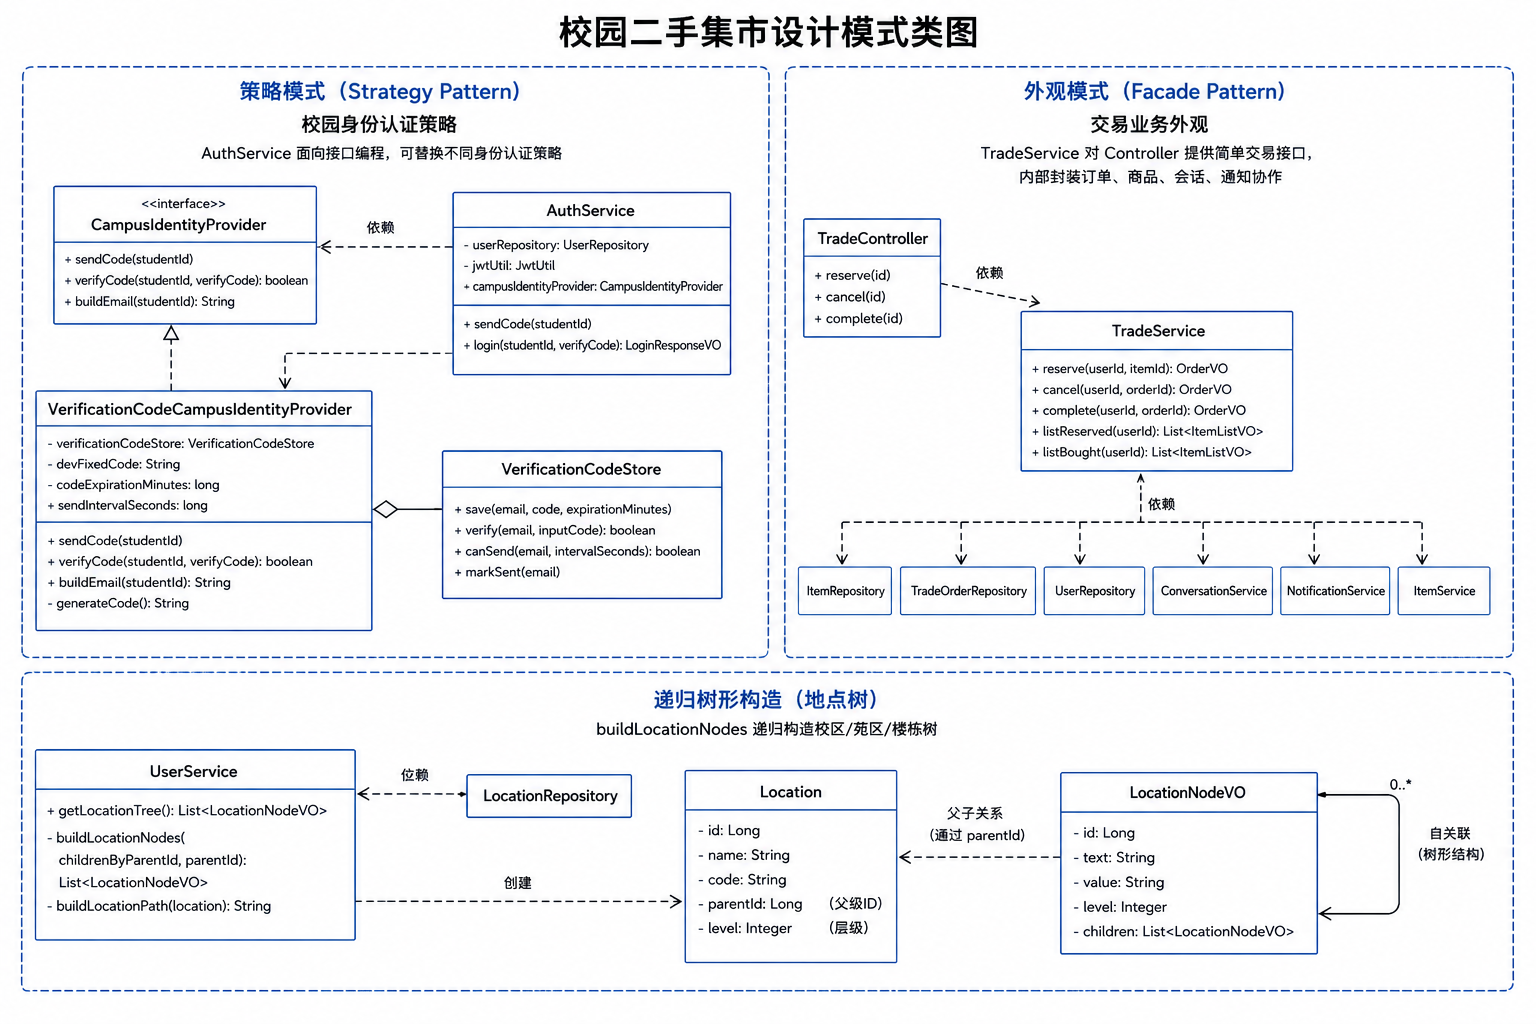
\includegraphics[width=0.95\textwidth]{shejimoshi.png}
  \caption{设计模式类图}
  \label{fig:design-patterns}
\end{figure}

\subsubsection{策略模式}
策略模式体现在校园身份认证模块中。系统定义了 \texttt{CampusIdentityProvider} 接口，抽象出发送验证码、校验验证码和生成校园邮箱地址等行为；当前实现类为 \texttt{VerificationCodeCampusIdentityProvider}，它通过 \texttt{VerificationCodeStore} 保存和验证验证码。认证服务 \texttt{AuthService} 面向 \texttt{CampusIdentityProvider} 接口编程，而不是直接依赖某一种验证码实现。

这种设计的好处是身份认证方式可以替换。例如课程演示阶段使用固定验证码或内存验证码存储，后续正式环境可以替换为校园邮箱验证码、统一身份认证或短信认证，只要新的实现类仍然实现 \texttt{CampusIdentityProvider} 接口，\texttt{AuthService} 的登录逻辑就不需要大规模修改。因此，该模块符合策略模式“定义一系列算法，将它们封装起来并使它们可以互相替换”的思想。

\subsubsection{外观模式思想}
交易业务中体现了外观模式思想。前端或 Controller 只需要调用 \texttt{TradeService} 提供的 \texttt{reserve}、\texttt{cancel}、\texttt{complete} 等方法，就可以完成商品预定、取消预定和确认完成交易。实际上，这些操作内部会涉及多个对象和组件：用户查询、商品状态检查、订单创建或更新、悲观锁控制、会话创建、通知生成以及列表 VO 转换。

\texttt{TradeService} 对外提供了简洁的交易接口，对内封装了复杂的对象协作。这样 Controller 不需要了解订单表如何保存、商品状态如何变化、通知何时生成，也不需要直接操作多个 Repository 和 Service。该设计降低了接口层复杂度，也使交易规则集中在一个服务类中，便于后续修改预定超时释放、卖家拒绝预定或管理员介入等功能。

\subsubsection{递归树形构造}
地点选择功能使用了递归树形构造思想。系统中的 \texttt{Location} 对象通过 \texttt{parentId} 表示校区、苑区、楼栋之间的父子关系，\texttt{UserService.getLocationTree()} 会先按父节点分组，再调用 \texttt{buildLocationNodes()} 递归生成 \texttt{LocationNodeVO} 树。每个 \texttt{LocationNodeVO} 都包含 \texttt{children} 列表，从而形成前端级联选择器所需的数据结构。

递归方式适合处理层级不固定或未来可能扩展的地点数据。如果后续新增校区、楼栋或更细的楼层节点，只需要维护 Location 数据，不需要重写前端地点选择结构。虽然递归不是 GoF 设计模式之一，但它是本项目需求建模和对象转换中重要的设计思想。

\subsubsection{模式选择说明}
本项目没有将适配器模式和桥接模式作为主要设计模式。适配器模式通常用于将已有不兼容接口转换为目标接口，而当前项目中的身份认证接口是主动抽象出来的策略接口，并不是为了适配已有旧接口；桥接模式强调抽象和实现两个维度独立变化，当前项目没有明显的双维度继承结构。因此，将本项目概括为“策略模式为主，外观模式思想和递归构造为辅”更符合实际代码。

\subsection{关键业务实现}
本项目的关键业务主要包括商品发布与搜索、商品预定与并发控制、私信会话和系统通知。

\subsubsection{商品发布与搜索}
商品发布由前端发布页收集图片、标题、分类、成色、价格、地点和描述，后端 \texttt{ItemService.createItem()} 负责校验用户资料是否完善、地点编码是否存在，并将首张图片设置为封面。商品图片通过 \texttt{ItemImage} 保存多图列表，使用 \texttt{sortOrder} 保持展示顺序。商品删除采用软删除方式，设置删除标记并将状态改为“已下架”，避免历史订单或会话引用失效。

商品列表查询使用 JPA Specification 动态构造条件。默认情况下只返回未删除且状态为“在售”的商品；如果传入分类、关键词或状态参数，则按对应条件过滤。关键词搜索覆盖商品标题、描述和卖家昵称，使买家可以通过商品名称或卖家信息快速定位目标商品。

\subsubsection{预定交易与并发控制}
商品预定是系统中最关键的业务流程。图 \ref{fig:reserve-flow} 和图 \ref{fig:reserve-sequence} 分别展示了预定流程和对象交互时序。

\begin{figure}[H]
  \centering
  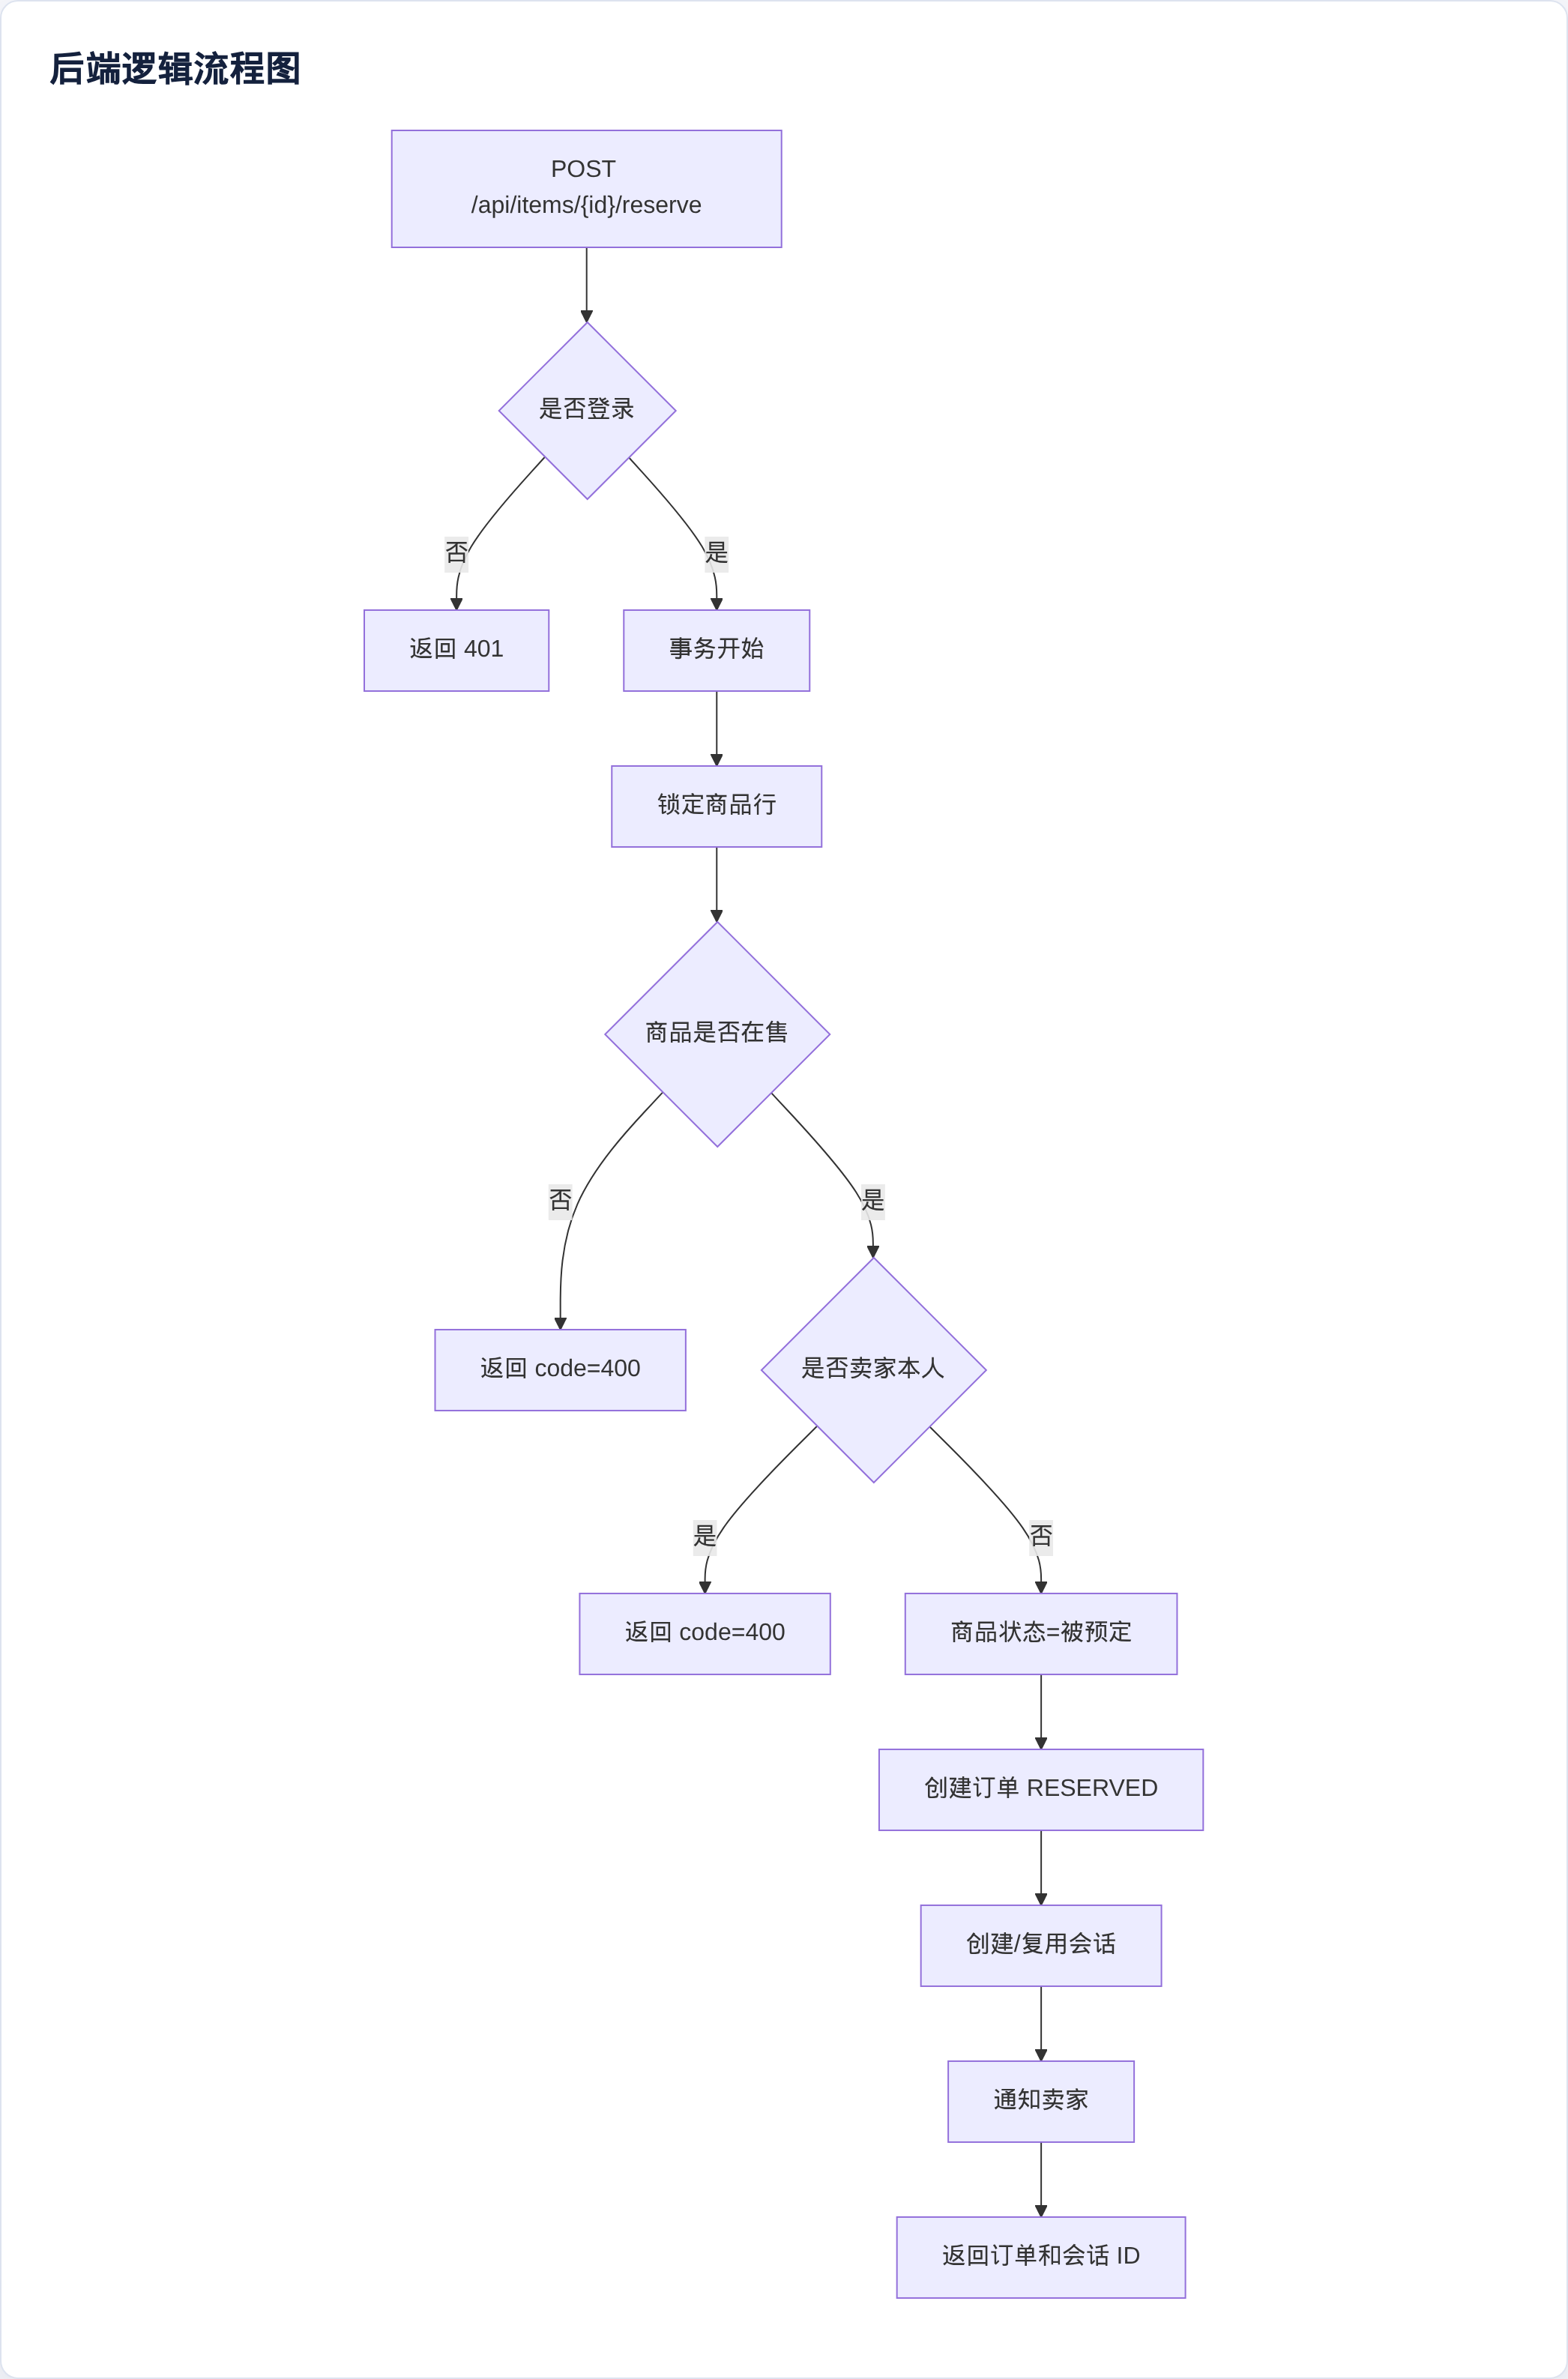
\includegraphics[width=0.85\textwidth]{backend-b-reserve-flow.png}
  \caption{商品预定业务流程图}
  \label{fig:reserve-flow}
\end{figure}

\begin{figure}[H]
  \centering
  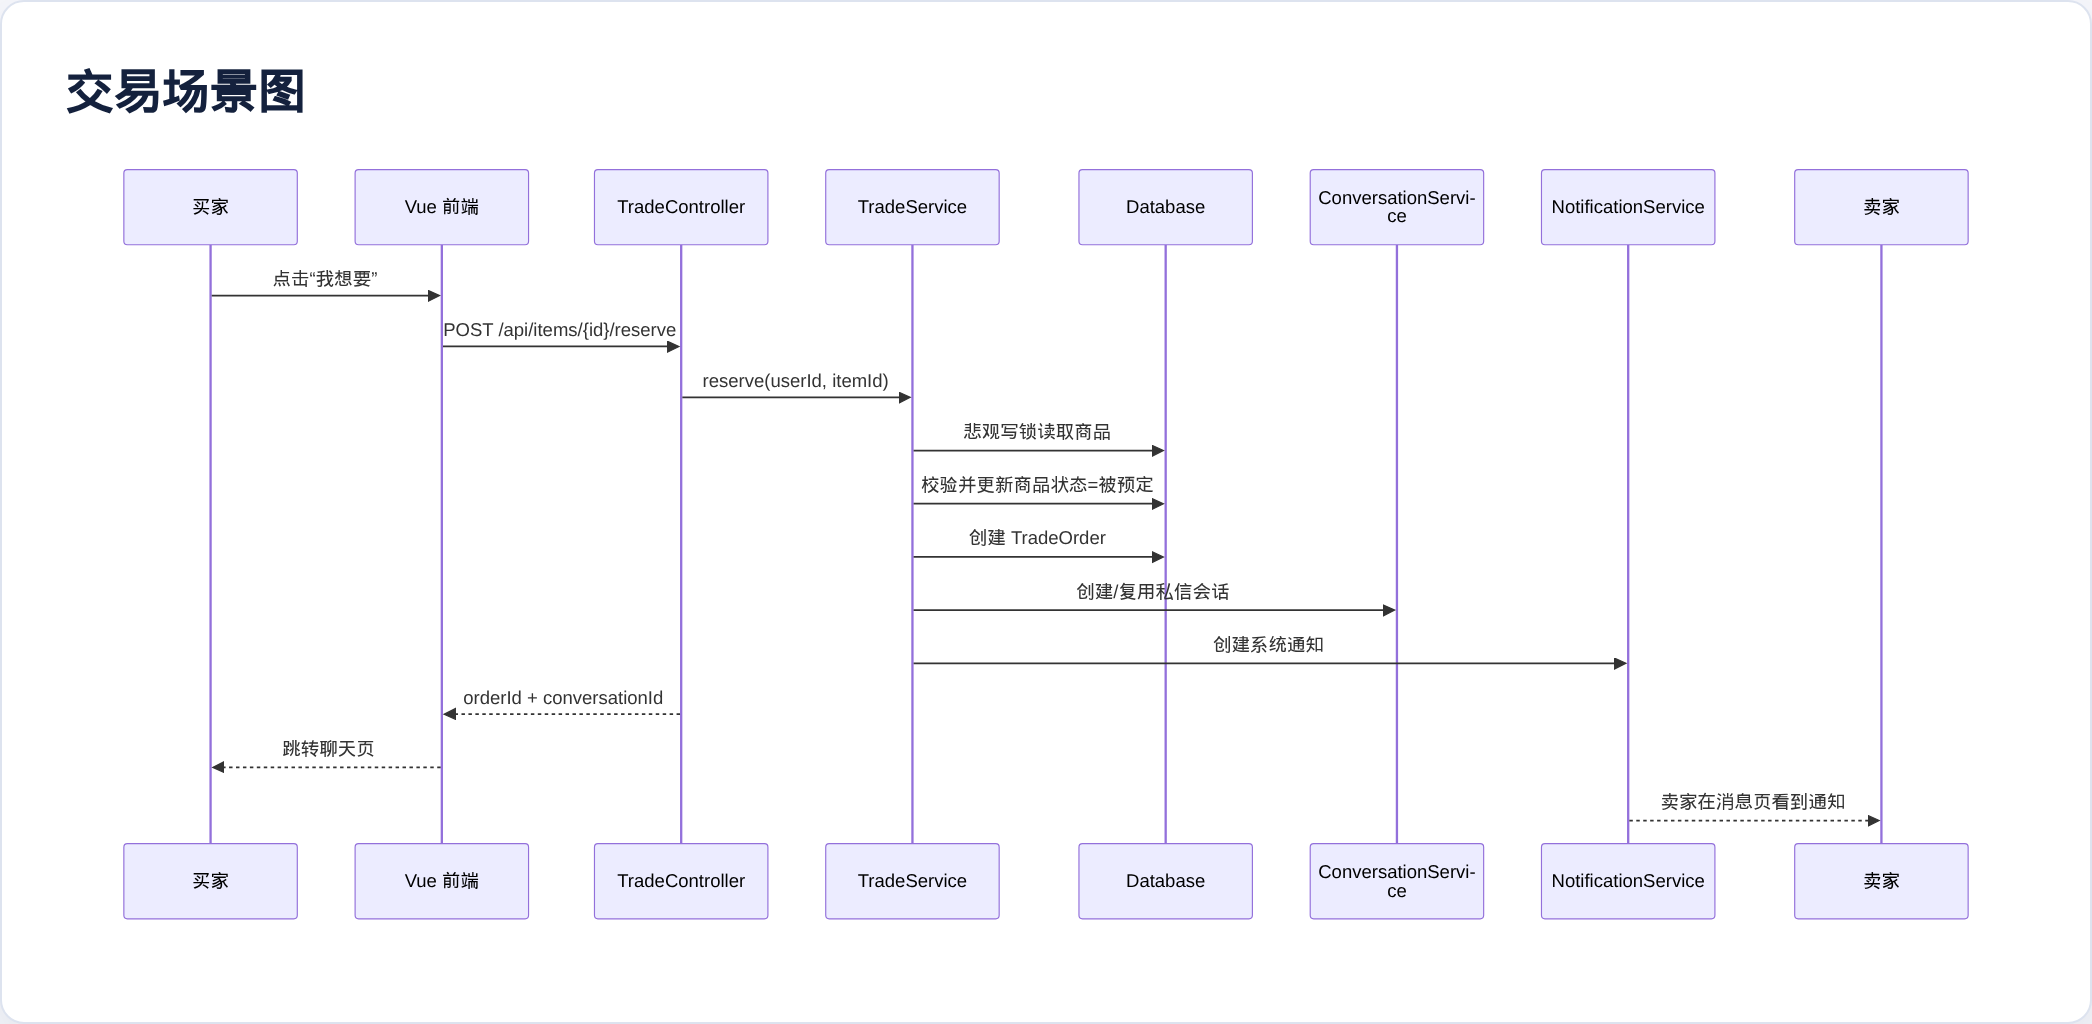
\includegraphics[width=0.9\textwidth]{backend-b-reserve-sequence.png}
  \caption{商品预定时序图}
  \label{fig:reserve-sequence}
\end{figure}

预定接口由 \texttt{TradeService.reserve()} 实现。该方法首先查询当前买家和目标商品，并使用 \texttt{findByIdForUpdate()} 对商品记录加悲观写锁；然后检查买家不能是卖家本人，商品必须处于“在售”状态；校验通过后，将商品状态改为“被预定”，创建 RESERVED 订单，创建或复用买卖双方的会话，并向卖家生成系统通知。悲观锁保证多个买家同时预定同一商品时，只有第一个完成状态修改的请求成功，其余请求会在状态检查阶段被拒绝。

\subsubsection{私信与通知}
私信功能由 \texttt{ConversationService} 实现。系统以商品、买家、卖家三元组唯一确定一个会话，避免同一商品重复创建多个会话。消息发送时，系统会记录发送者、接收者、正文、引用消息和创建时间，并更新会话的最后消息和接收方未读数量。消息撤回限制为发送者本人且 2 分钟内，防止任意撤回他人消息或长时间后修改聊天记录。

通知功能由 \texttt{NotificationService} 实现。交易服务在预定、取消和完成交易时调用通知服务创建系统通知，通知可关联商品和会话，前端消息页可以据此跳转到相关交易上下文。通知支持单条已读和全部已读，未读数量会和私信未读数一起组成消息角标。

\section{验收与发布}

\subsection{测试策略}
本项目的验收目标是验证系统能够稳定支撑校园二手交易核心闭环，即用户可以完成登录、资料完善、商品发布、浏览搜索、收藏私信、预定商品、取消或完成交易以及接收系统通知。测试策略采用“后端自动化测试 + 前端构建验证 + 性能压测 + 手工验收流程”的组合方式，既覆盖接口和业务规则，也覆盖课程演示所需的页面流程。

后端测试以 Spring Boot Test、JUnit 5、MockMvc 和 H2 测试数据库为基础，直接经过 Controller、Service、Repository 和数据库链路，属于集成测试而非单纯单元测试。自动化测试覆盖认证、用户资料、地点树、商品 CRUD、图片上传、收藏、私信、通知、交易状态流转、异常输入、越权访问和并发预定等场景。对于交易相关功能，测试重点不是只验证接口能否返回成功，而是验证商品状态、订单状态、通知和权限规则是否符合需求。

前端测试以生产构建和人工验收为主。当前项目尚未引入 Playwright 等浏览器端 E2E 测试框架，因此前端通过 \texttt{npm run build} 验证依赖、语法和打包流程，通过人工操作验证登录、首页、详情、发布、消息和个人中心等页面能否串联。性能测试使用 \texttt{scripts/qa-load-test.js} 脚本，对商品列表、搜索、详情和并发预定接口进行压测，统计成功率、平均耗时、P95 和最大耗时。

\begin{table}[H]
  \centering
  \caption{测试策略说明}
  \begin{tabular}{p{3cm}p{5.2cm}p{5.5cm}}
    \toprule
    测试类型 & 测试内容 & 验收重点 \\
    \midrule
    后端集成测试 & 认证、用户、商品、上传、收藏、交易、私信、通知 & 接口返回、数据库状态、业务规则和统一错误码是否正确 \\
    异常场景测试 & 非法输入、越权操作、已下架商品、重复状态流转 & 系统能否返回明确业务错误，且不破坏已有数据 \\
    并发测试 & 多个买家同时预定同一商品 & 只能有一个买家成功，避免一物多卖 \\
    前端构建验证 & Vue/Vite 生产构建 & 前端依赖、组件代码和构建配置是否可用 \\
    性能压测 & 商品列表、搜索、详情、并发预定接口 & 成功率、平均耗时、P95 是否满足课程演示规模 \\
    手工验收 & 登录、发布、浏览、私信、预定、完成交易完整流程 & 页面流程是否能支撑现场演示和用户操作 \\
    \bottomrule
  \end{tabular}
\end{table}

\subsection{测试用例}
项目测试用例已在 \texttt{docs/QA\_TEST\_CASES.md} 中按认证、商品、交易、私信、通知、前端验收和性能测试分类整理。表 \ref{tab:main-test-cases} 选取其中具有代表性的核心测试用例，覆盖正常流程、异常流程、权限控制和并发可靠性。

\begin{longtable}{p{2.4cm}p{3.5cm}p{4.5cm}p{3cm}}
  \caption{主要测试用例}\label{tab:main-test-cases} \\
  \toprule
  用例编号 & 测试点 & 操作步骤 & 预期结果 \\
  \midrule
  \endfirsthead
  \toprule
  用例编号 & 测试点 & 操作步骤 & 预期结果 \\
  \midrule
  \endhead
  AUTH-001 & 未登录保护 & 不携带认证信息访问用户资料接口 & 返回 HTTP 401，业务码为 401 \\
  USER-002 & 完善个人资料 & 登录后提交昵称、微信号和地点编码 & 用户资料保存成功，\texttt{isProfileComplete=true} \\
  ITEM-001 & 发布商品 & 资料完整卖家提交标题、分类、价格、地点和图片 & 返回商品 ID 和商品详情，商品状态为“在售” \\
  ITEM-008 & 商品越权修改 & 非发布者尝试修改他人商品 & 返回 \texttt{code=403}，商品数据不被修改 \\
  UPLOAD-002 & 非图片上传 & 上传 txt 等非图片文件 & 返回 \texttt{code=400}，拒绝保存文件 \\
  TRADE-001 & 买家预定商品 & 买家对在售商品调用预定接口 & 创建 RESERVED 订单，商品状态变为“被预定” \\
  TRADE-004 & 买家确认完成 & 买家尝试调用确认完成接口 & 返回 \texttt{code=403}，只有卖家可以确认完成 \\
  TRADE-010 & 并发预定 & 多个买家线程同时预定同一商品 & 仅 1 个请求成功，其余返回业务拒绝 \\
  CHAT-003 & 发送私信 & 会话参与者发送文字消息 & 消息保存，接收方未读数加 1 \\
  CHAT-006 & 路人读取会话 & 非会话参与者请求消息列表 & 返回 \texttt{code=403}，不能查看他人会话 \\
  NOTIFY-001 & 预定通知 & 买家预定商品后卖家查询通知 & 卖家收到 RESERVE\_CREATED 类型通知 \\
  FE-001 & 前端构建 & 在前端目录执行 \texttt{npm run build} & 构建成功，生成 \texttt{frontend/dist} 产物 \\
  \bottomrule
\end{longtable}

\subsection{测试结果}
根据项目测试报告 \texttt{docs/QA\_TEST\_REPORT.md}，当前版本已完成后端自动化测试、前端生产构建和性能压测。后端自动化测试执行命令为 \texttt{cd backend \&\& ./mvnw test}，测试结果为 \texttt{Tests run: 15, Failures: 0, Errors: 0, Skipped: 0}，构建结果为 \texttt{BUILD SUCCESS}。测试覆盖 Spring Boot 上下文启动、认证与用户资料、商品 CRUD、图片上传、交易状态流转、收藏、私信、通知、开发期认证开关、异常场景和并发预定。

前端构建执行命令为 \texttt{cd frontend \&\& npm run build}，构建成功并生成 \texttt{frontend/dist} 目录。构建摘要显示 Vite 完成 314 个模块转换，并输出 \texttt{index.html}、CSS 和 JS 资源。该结果说明前端依赖、组件代码、路由和打包配置能够满足本地演示和静态资源部署要求。

性能压测通过 \texttt{scripts/qa-load-test.js} 执行，覆盖商品列表、商品搜索、商品详情和并发预定四类场景。列表、搜索和详情接口成功率均为 100\%；并发预定场景中 10 个请求只有 1 个买家成功，其余 9 个请求返回业务拒绝，符合“一件商品只能被一个买家预定”的设计目标。

\begin{table}[H]
  \centering
  \caption{测试执行结果汇总}
  \begin{tabular}{p{3.2cm}p{4.8cm}p{5.2cm}}
    \toprule
    测试项 & 执行结果 & 结论 \\
    \midrule
    后端自动化测试 & 15 个测试全部通过，0 失败，0 错误 & 后端核心接口、状态流转、异常和并发规则通过验证 \\
    前端生产构建 & Vite 构建成功，生成 \texttt{frontend/dist} & 前端代码可构建，可用于本地预览或静态部署 \\
    商品列表压测 & 100 次请求成功率 100\%，平均耗时约 6.9ms，P95 约 16.9ms & 满足课程演示规模下的响应要求 \\
    商品搜索压测 & 100 次请求成功率 100\%，平均耗时约 5.5ms，P95 约 11.8ms & 搜索接口响应稳定 \\
    商品详情压测 & 100 次请求成功率 100\%，平均耗时约 10.6ms，P95 约 26.1ms & 详情接口响应稳定 \\
    并发预定压测 & 10 个并发请求中 1 个成功、9 个业务拒绝 & 并发预定结果符合预期，未出现一物多卖 \\
    \bottomrule
  \end{tabular}
\end{table}

本轮验收仍存在若干后续风险：第一，当前并发测试主要在 H2 环境完成，MySQL 部署后仍应补充相同并发测试；第二，前端尚未引入自动化 E2E 测试，页面兼容性和视觉回归主要依赖人工检查；第三，举报审核、管理员处理和预定超时自动释放不属于当前交付闭环，已记录为后续迭代项。总体来看，在当前实现范围内，系统已经满足课程演示和基础验收要求。

\subsection{发布说明}
本项目当前发布方式以本地演示发布为主，适合课程答辩、教师验收和小组成员联调。后端默认使用 H2 内存数据库，无需手动创建数据库；启动时会初始化地点树和演示数据。前端通过 Vite 开发服务器运行，并将 \texttt{/api} 和 \texttt{/uploads} 请求代理到后端。若需要接入 MySQL，可使用后端的 \texttt{mysql} profile，并根据本机数据库修改用户名、密码和连接地址。

本地发布环境要求如下：Java 17、Maven Wrapper、Node.js、npm 和现代浏览器。后端默认端口为 8080，前端默认端口为 5173。开发演示验证码为 \texttt{123456}，首次登录后需要完成昵称、地点和微信号等资料填写。

\begin{table}[H]
  \centering
  \caption{本地发布与验收命令}
  \begin{tabular}{p{4.4cm}p{8.6cm}}
    \toprule
    操作 & 命令或说明 \\
    \midrule
    启动后端 & 进入 \texttt{backend} 目录，执行 \texttt{./mvnw spring-boot:run}，服务地址为 \texttt{http://localhost:8080} \\
    启动前端 & 进入 \texttt{frontend} 目录，执行 \texttt{npm run dev}，页面地址通常为 \texttt{http://localhost:5173} \\
    后端测试 & 进入 \texttt{backend} 目录，执行 \texttt{./mvnw test} \\
    前端构建 & 进入 \texttt{frontend} 目录，执行 \texttt{npm run build}，产物输出到 \texttt{frontend/dist} \\
    性能压测 & 后端启动后，在项目根目录执行 \texttt{node scripts/qa-load-test.js} \\
    MySQL 模式 & 使用后端 \texttt{application-mysql.yml}，通过 \texttt{mysql} profile 切换数据源 \\
    \bottomrule
  \end{tabular}
\end{table}

本次交付物包括：前端源码、后端源码、数据库结构说明、自动化测试代码、压测脚本、用户手册与维护说明、测试计划、测试用例、测试报告、系统设计图和最终实验报告。验收时建议按以下顺序进行：先启动后端并访问健康检查接口，再启动前端完成登录和资料完善；随后由卖家发布商品，买家搜索商品、进入详情、发起私信并预定；最后由卖家确认完成交易，并检查买家订单列表和系统通知。该流程能够覆盖系统的主要功能闭环。

\section{运行与维护}

\subsection{运行环境}
本项目采用前后端分离方式运行。后端依赖 Java 17 和 Maven Wrapper，前端依赖 Node.js、npm 和现代浏览器。开发演示环境默认使用 H2 内存数据库，因此不需要提前安装数据库服务；若需要更接近正式部署环境，可以切换到 MySQL profile，并使用 MySQL 作为持久化数据库。

\begin{table}[H]
  \centering
  \caption{运行环境要求}
  \begin{tabular}{p{3.2cm}p{4.2cm}p{5.8cm}}
    \toprule
    环境项 & 推荐配置 & 说明 \\
    \midrule
    后端运行环境 & Java 17 & Spring Boot 后端运行和测试所需环境 \\
    后端构建工具 & Maven Wrapper & 项目自带 \texttt{mvnw}，无需全局安装 Maven \\
    前端运行环境 & Node.js、npm & 用于安装依赖、启动 Vite 和执行前端构建 \\
    前端框架 & Vue 3、Vite、Vant、Tailwind CSS & 构建移动端风格 Web 页面 \\
    默认数据库 & H2 内存数据库 & 适合本地快速启动、课程演示和自动化测试 \\
    可选数据库 & MySQL & 通过 \texttt{mysql} profile 切换，用于后续部署验证 \\
    浏览器 & Chrome、Edge、Safari 或手机浏览器 & 用于访问前端页面和演示系统功能 \\
    默认端口 & 后端 8080，前端 5173 & Vite 会将 \texttt{/api} 和 \texttt{/uploads} 代理到后端 \\
    \bottomrule
  \end{tabular}
\end{table}

\subsection{启动与停止}
本地启动时建议先启动后端，再启动前端。后端默认读取 \texttt{application.yml}，使用 H2 内存数据库和开发演示验证码；前端启动后通过 Vite 代理访问后端 API。停止系统时，可在对应终端使用 \texttt{Ctrl+C} 停止前端和后端进程。

\begin{table}[H]
  \centering
  \caption{系统启动与停止}
  \begin{tabular}{p{3.2cm}p{5.5cm}p{4.5cm}}
    \toprule
    操作 & 命令 & 说明 \\
    \midrule
    启动后端 & \texttt{cd backend}；\texttt{./mvnw spring-boot:run} & 后端默认运行在 \texttt{http://localhost:8080} \\
    启动前端 & \texttt{cd frontend}；\texttt{npm run dev} & 前端默认运行在 \texttt{http://localhost:5173} \\
    后端测试 & \texttt{cd backend}；\texttt{./mvnw test} & 执行后端自动化测试和回归测试 \\
    前端构建 & \texttt{cd frontend}；\texttt{npm run build} & 生成 \texttt{frontend/dist} 构建产物 \\
    性能压测 & \texttt{node scripts/qa-load-test.js} & 需要先启动后端服务 \\
    停止服务 & 终端中按 \texttt{Ctrl+C} & 分别停止前端和后端进程 \\
    \bottomrule
  \end{tabular}
\end{table}

常见启动问题主要包括端口占用、前端依赖未安装、后端 Java 版本不匹配和压测时后端未启动。如果前端 5173 端口被占用，Vite 可能自动切换到其他端口；后端默认 CORS 配置允许 localhost 多端口访问。如果登录失败，应确认已点击“获取验证码”，并在开发环境使用固定验证码 \texttt{123456}。

\subsection{数据维护}
开发和测试环境默认使用 H2 内存数据库，系统启动时由初始化逻辑创建地点树、默认用户和演示数据。H2 的优点是启动快、环境依赖少，适合课程展示；缺点是服务重启后内存数据会重置，不适合保存长期真实数据。

若需要使用 MySQL，需要维护 \texttt{backend/src/main/resources/application-mysql.yml} 中的数据库连接配置，并根据本机环境设置用户名、密码和数据库地址。切换到 MySQL 后，应确认 \texttt{app.security.dev-auth-enabled=false}，避免正式环境继续使用开发期 Header。数据库表结构可参考 \texttt{backend/src/main/resources/db/schema.sql}，切换后应重新执行后端自动化测试和并发预定测试。

上传图片默认保存在后端配置的 \texttt{uploads} 目录中。维护时需要注意三点：第一，定期清理已经下架或测试过程中产生的无用图片；第二，保证目录权限只允许后端服务写入；第三，正式部署时可将图片迁移到独立对象存储或受控静态资源目录，降低应用服务器磁盘压力。

\subsection{安全维护}
安全维护重点是区分开发环境和正式环境。开发环境为了便于演示，允许固定验证码和 \texttt{X-Dev-User-Id} Header；正式环境必须关闭开发期认证开关，替换默认 JWT 密钥，并接入真实校园邮箱验证码或统一身份认证服务。

\begin{table}[H]
  \centering
  \caption{安全维护要求}
  \begin{tabular}{p{3.2cm}p{9.4cm}}
    \toprule
    维护项 & 要求 \\
    \midrule
    JWT 密钥 & 正式环境必须替换默认密钥，密钥长度和复杂度应满足签名算法要求，不能提交到公开仓库 \\
    开发期 Header & 正式环境必须关闭 \texttt{app.security.dev-auth-enabled}，防止绕过登录流程 \\
    验证码机制 & 开发期固定验证码仅用于演示，正式环境应接入真实校园邮箱或统一身份认证 \\
    文件上传 & 继续限制图片大小、类型、扩展名和保存路径，必要时增加图片压缩和安全扫描 \\
    权限校验 & 商品、订单、会话、消息和通知操作都必须在后端校验当前用户身份 \\
    错误响应 & 不向前端暴露异常堆栈和服务器路径，统一返回业务错误码和用户可理解的提示 \\
    CORS 来源 & 正式部署时将允许来源从 localhost 收紧为实际前端域名 \\
    \bottomrule
  \end{tabular}
\end{table}

\subsection{性能维护}
当前版本可以满足课程演示和小规模试点，但随着商品数量、图片数量和聊天消息增加，仍需要持续关注列表查询、搜索、图片加载和消息刷新性能。性能维护方向如表 \ref{tab:performance-maintenance} 所示。

\begin{table}[H]
  \centering
  \caption{性能维护建议}
  \label{tab:performance-maintenance}
  \begin{tabular}{p{3.2cm}p{9.4cm}}
    \toprule
    场景 & 优化建议 \\
    \midrule
    商品列表变慢 & 增加分页或无限滚动，避免一次返回全部商品；为商品状态、分类和创建时间增加索引 \\
    搜索变慢 & 对标题、分类、状态等字段建立索引，必要时接入专门搜索服务 \\
    商品详情变慢 & 减少重复查询地点路径和图片数据，可增加缓存或批量查询优化 \\
    图片加载慢 & 生成缩略图，压缩上传图片，使用静态资源缓存或对象存储 \\
    消息数据增长 & 消息列表增加分页，避免一次加载全部历史消息 \\
    未读刷新频繁 & 小规模阶段可轮询，后续可引入 WebSocket 或 Server-Sent Events \\
    并发预定冲突多 & 保留事务和悲观锁，部署 MySQL 后重复执行并发压测验证锁行为 \\
    \bottomrule
  \end{tabular}
\end{table}

\subsection{后续迭代计划}
本版本已经完成校园二手交易核心闭环，但距离真实长期运营仍有若干增强方向。后续迭代计划见表 \ref{tab:future-plan}。

\begin{table}[H]
  \centering
  \caption{后续迭代计划}
  \label{tab:future-plan}
  \begin{tabular}{p{3.2cm}p{9.4cm}}
    \toprule
    迭代方向 & 说明 \\
    \midrule
    管理员后台 & 增加管理员角色、商品审核、用户管理和违规处理入口 \\
    举报审核 & 新增举报实体、举报接口、处理状态和管理员审核记录 \\
    预定超时释放 & 商品被预定后若长时间未完成交易，可由定时任务自动恢复为在售 \\
    真实校园认证 & 接入校园邮箱、统一身份认证或学校账号系统，替代开发期固定验证码 \\
    浏览器 E2E 测试 & 使用 Playwright 覆盖登录、发布、搜索、私信、预定和完成交易流程 \\
    消息实时推送 & 将当前请求式未读刷新升级为 WebSocket 或 SSE，提高消息即时性 \\
    部署监控 & 增加接口日志、错误率、响应时间、数据库连接和磁盘容量监控 \\
    数据备份 & 为 MySQL 数据库和上传图片目录建立定期备份与恢复方案 \\
    \bottomrule
  \end{tabular}
\end{table}

\section{总结}
本项目围绕校园二手物品交易场景，完成了一个前后端分离的 Web 平台。系统实现了从用户登录、资料完善、商品发布、浏览搜索、收藏私信、商品预定、取消预定、确认完成到系统通知的核心交易闭环。前端采用 Vue 3、Vite、Vant 和 Tailwind CSS 构建移动端风格页面；后端采用 Spring Boot、Spring Security、JWT、Spring Data JPA 和 H2/MySQL 构建 REST API 和业务服务。项目代码按照前端组件、API 封装、后端 Controller、Service、Repository、Entity 和 DTO 分层组织，具备较清晰的模块边界。

从软件工程过程看，小组按照课程周期完成了可行性分析、需求获取与建模、原型设计、系统架构设计、组件图、部署图、安全设计、程序开发、测试验收和维护计划。项目在需求分析中使用干系人分析确定买家、卖家、课程评审者、开发小组和维护者的需求；在设计阶段选择客户端/服务器和三层体系结构；在实现阶段使用策略模式、外观模式思想和递归树形构造；在测试阶段通过自动化测试、异常场景测试、并发预定测试、前端构建和性能压测验证系统质量。

本项目的主要收获包括三点。第一，团队加深了对前后端分离系统的理解，能够通过统一 REST API 和数据传输对象协调页面与后端业务。第二，团队认识到状态流转和权限校验是交易类系统的关键，不能只依赖前端按钮控制，而必须在后端通过事务、锁和业务规则保证一致性。第三，团队通过测试计划、测试用例和测试报告体会到软件质量保证并不是最后一步补充工作，而应贯穿需求、设计和实现全过程。

项目仍存在不足。首先，当前系统主要面向课程演示和小规模试点，尚未实现管理员后台、举报审核、预定超时自动释放和真实校园统一认证。其次，前端自动化测试不足，页面兼容性和端到端流程主要依赖手工验收。再次，H2 开发环境与 MySQL 正式环境在锁行为、性能和配置方面可能存在差异，后续部署前仍需补充真实数据库环境下的回归测试和压测。

总体而言，\projectname{}已经达到了课程实验的预期目标：系统功能闭环完整，技术路线清晰，需求、设计、实现、测试和维护文档较为完整，能够支撑最终演示和报告验收。后续若继续迭代，可在平台治理、实时消息、生产部署和自动化测试方面进一步完善，使其从课程项目逐步接近可试点运行的校园服务。

\newpage
\appendix

\section{附录：项目运行命令}
本附录汇总项目常用运行、测试和构建命令。Windows 环境可将 \texttt{./mvnw} 替换为 \texttt{mvnw.cmd}。

\begin{longtable}{p{4cm}p{9cm}}
  \caption{项目常用命令} \\
  \toprule
  目的 & 命令 \\
  \midrule
  \endfirsthead
  \toprule
  目的 & 命令 \\
  \midrule
  \endhead
  启动后端 & \texttt{cd backend}；\texttt{./mvnw spring-boot:run} \\
  运行后端测试 & \texttt{cd backend}；\texttt{./mvnw test} \\
  使用 MySQL profile 启动后端 & \texttt{cd backend}；\texttt{./mvnw spring-boot:run -Dspring-boot.run.profiles=mysql} \\
  安装前端依赖 & \texttt{cd frontend}；\texttt{npm ci} \\
  启动前端开发服务器 & \texttt{cd frontend}；\texttt{npm run dev} \\
  构建前端生产产物 & \texttt{cd frontend}；\texttt{npm run build} \\
  预览前端构建产物 & \texttt{cd frontend}；\texttt{npm run preview} \\
  执行默认压测脚本 & \texttt{node scripts/qa-load-test.js} \\
  调整压测规模 & \texttt{BASE\_URL=http://localhost:8080 TOTAL=200 CONCURRENCY=20 node scripts/qa-load-test.js} \\
  查看后端健康检查 & 浏览器访问 \texttt{http://localhost:8080/api/health} \\
  访问前端页面 & 浏览器访问 \texttt{http://localhost:5173} \\
  \bottomrule
\end{longtable}

\section{附录：接口清单}
完整接口测试清单见 \texttt{docs/API\_TEST\_CHECKLIST.md}。该文档列出了认证、用户资料、地点树、商品、上传、交易、收藏、私信和通知等接口的请求方式、请求路径、验证点和通过情况。表 \ref{tab:appendix-api-summary} 给出接口分类摘要。

\begin{longtable}{p{3.2cm}p{4cm}p{6cm}}
  \caption{接口清单摘要}\label{tab:appendix-api-summary} \\
  \toprule
  分类 & 代表接口 & 说明 \\
  \midrule
  \endfirsthead
  \toprule
  分类 & 代表接口 & 说明 \\
  \midrule
  \endhead
  认证 & \texttt{POST /api/auth/send-code}、\texttt{POST /api/auth/login} & 验证码发送和登录换取 JWT \\
  用户与地点 & \texttt{GET /api/users/me}、\texttt{PUT /api/users/me}、\texttt{GET /api/locations/tree} & 当前用户资料和地点树 \\
  商品 & \texttt{GET /api/items}、\texttt{POST /api/items}、\texttt{GET /api/items/\{id\}} & 商品列表、发布和详情 \\
  上传 & \texttt{POST /api/upload/image} & 上传商品图片并返回访问路径 \\
  收藏 & \texttt{POST /api/items/\{id\}/favorite}、\texttt{GET /api/favorites} & 收藏、取消收藏和收藏列表 \\
  交易 & \texttt{POST /api/items/\{id\}/reserve}、\texttt{POST /api/orders/\{id\}/cancel}、\texttt{POST /api/orders/\{id\}/complete} & 预定、取消和完成交易 \\
  私信 & \texttt{GET /api/conversations}、\texttt{POST /api/conversations/\{id\}/messages}、\texttt{POST /api/messages/\{id\}/recall} & 会话列表、消息发送和撤回 \\
  通知 & \texttt{GET /api/notifications}、\texttt{POST /api/notifications/read-all} & 通知列表和全部已读 \\
  未读汇总 & \texttt{GET /api/messages/unread-summary} & 私信、通知和总未读数 \\
  健康检查 & \texttt{GET /api/health} & 后端服务运行状态检查 \\
  \bottomrule
\end{longtable}

\section{附录：测试报告}
完整测试计划、测试用例和测试执行记录位于 \texttt{docs/} 目录：

\begin{itemize}
  \item \texttt{QA\_TEST\_PLAN.md}：说明测试目标、范围、环境、策略、进入和退出标准。
  \item \texttt{QA\_TEST\_CASES.md}：列出认证、商品、交易、私信、通知、前端和性能测试用例。
  \item \texttt{QA\_TEST\_REPORT.md}：记录后端自动化测试、前端构建和性能压测结果。
  \item \texttt{API\_TEST\_CHECKLIST.md}：提供手工接口验收清单。
\end{itemize}

根据测试报告，当前版本后端自动化测试通过，前端构建通过，性能压测中列表、搜索和详情接口成功率为 100\%，并发预定场景符合“只有一个买家成功”的预期。举报审核、管理员后台、预定超时释放和前端 E2E 测试作为后续迭代项记录。



\end{document}
